\documentclass[11pt]{article}
\usepackage[margin=1in]{geometry}
\usepackage{amsmath,amssymb,amsthm,mathtools,bm}
\usepackage{enumitem,booktabs,graphicx,xcolor}
\usepackage[numbers,sort&compress]{natbib}
\usepackage[colorlinks=true,linkcolor=blue!50!black,citecolor=blue!50!black,urlcolor=blue!50!black]{hyperref}
\usepackage[capitalise]{cleveref}

\newtheorem{theorem}{Theorem}
\newtheorem{lemma}[theorem]{Lemma}
\newtheorem{proposition}[theorem]{Proposition}
\newtheorem{corollary}[theorem]{Corollary}
\newtheorem{conjecture}[theorem]{Conjecture}
\theoremstyle{definition}
\newtheorem{definition}[theorem]{Definition}
\newtheorem{assumption}[theorem]{Assumption}
\newtheorem{procedure}[theorem]{Procedure}
\theoremstyle{remark}
\newtheorem{remark}[theorem]{Remark}
\newtheorem{example}[theorem]{Example}
\crefname{procedure}{Procedure}{Procedures}
\crefname{assumption}{Assumption}{Assumptions}

\newcommand{\R}{\mathbb{R}}
\newcommand{\E}{\mathbb{E}}
\newcommand{\N}{\mathcal{N}}
\newcommand{\T}{\mathcal{T}}
\newcommand{\F}{\mathfrak{F}}
\newcommand{\cA}{\mathcal{A}}
\newcommand{\hy}{\hat{y}}
\newcommand{\diam}{\operatorname{diam}}
\newcommand{\tr}{\operatorname{tr}}
\newcommand{\Var}{\operatorname{Var}}
\newcommand{\lean}[1]{\textup{\small[Lean:~\texttt{\detokenize{#1}}]}}

\title{Cobweb Forests:\\ A Kolmogorov--Arnold Theory of Networks of Concept Hierarchies}
\author{Draft --- Karthik Singaravadivelan et al.\ (working notes)}
\date{\today}

\begin{document}
\maketitle

\begin{abstract}
The Kolmogorov--Arnold (KA) representation theorem states that every continuous
function of $n$ variables is a finite superposition of continuous functions of one
variable and addition, and Kolmogorov--Arnold Networks (KANs) turn that statement into
an architecture with learnable univariate functions on its edges.  We ask the two
analogous questions for Cobweb, the incremental concept-formation system whose
category utility measures the information its concepts carry about the features.
\emph{Representation:} is there a set of Cobweb trees that represents an arbitrary
continuous function?  \emph{Learnability:} does Cobweb's own learning
procedure---category utility and its four operators, with no gradients---learn it?
We formalise a \emph{Cobweb forest}: a directed acyclic graph of hybrid Cobweb trees in
which each tree reads raw features and the \emph{messages} of other trees---their
\emph{activations} (multi-node predictions of an attribute) and their \emph{labels}
(the concepts an input sorts to)---and one designated tree produces the output.
On representation we prove that a single tree is a universal approximator under the
implementation's prediction rules---all four weightings restricted to the leaves, and two
of them over all concepts (on a flat tree the other two keep a fixed bias, which a
hierarchy removes only slowly or not at all)---a
Cobweb--Kolmogorov--Arnold theorem (forests of two-input trees passing activations are
universal with $4n^2+4n$ trees, and one input per tree is not enough), that label forests
are universal, and that merging trees under a common root yields mixtures, not
compositions.  On learnability we prove that no Cobweb operator ever deletes a leaf,
which makes a learned tree, predicting with its count-weighted leaves, a universally
consistent regressor whatever structure category utility builds, and we introduce \emph{cognitive tasks}: what each tree
perceives (its \emph{cue}) and what it predicts and later observes (its
\emph{outcome}).  Under regularity conditions a forest learned by Cobweb converges to the
\emph{ideal forest} of its task assignment, which equals the target exactly when the assignment is
\emph{sufficient}; predicting the target at every tree is sufficient for
monotone-additive targets, predicting another view of the input is sufficient in a
Gaussian multi-view model whose target depends only on what the views share, and
categorization is sufficient whenever its cells shrink and stay few compared with the
sample and its smoothing vanishes fast enough, a requirement that grows with the dimension.  Tasks cannot be inferred locally---a sign construction makes a tree's
own data identical whether its input is necessary or irrelevant---but they can be
inferred consistently by verifying candidate tasks at the tree that composes them.  A cue
calculus maps associative, contextual, blocked and self-generated cues onto validities
of forest quantities and yields a procedure that designs a forest from held-out errors
alone.  The discrete cores of the statements are proved in Lean~4, an executable verifier
tests the statements against the implementation, and an independent reviewer, calibrated
on a copy with planted errors, audits the proofs.
\end{abstract}

\tableofcontents

%=====================================================================
\section{Introduction}
%=====================================================================

\paragraph{Kolmogorov--Arnold.}
For every $n\ge 2$ there are continuous functions $\varphi_{q,p}:[0,1]\to\R$
($q=0,\dots,2n$, $p=1,\dots,n$) such that every $f\in C([0,1]^n)$ can be written as
\begin{equation}\label{eq:ka}
  f(x_1,\dots,x_n)=\sum_{q=0}^{2n}\Phi_q\Bigl(\sum_{p=1}^{n}\varphi_{q,p}(x_p)\Bigr)
\end{equation}
with continuous outer functions $\Phi_q:\R\to\R$ that depend on~$f$
\citep{kolmogorov1957,arnold1957,lorentz1966,sprecher1965}.  The only genuinely
multivariate operation is addition.  The functions in \eqref{eq:ka} need not be
smooth---the inner functions can be chosen monotone, but in general the representation
cannot be made continuously differentiable---which long made \eqref{eq:ka} look
irrelevant to learning \citep{girosi1989}.  Kolmogorov--Arnold Networks \citep{liu2024kan} stack layers of
learnable univariate functions (B-splines on edges, sums at nodes) and prove an
approximation theorem whose rate does not depend on $n$ when $f$ has a \emph{smooth}
KA-type representation \citep[Thm.~2.1]{liu2024kan}.

\paragraph{Cobweb.}
Cobweb \citep{fisher1987} sorts each instance down a hierarchy of probabilistic
concepts and, at every node, applies whichever of four operators---add to the best
child, create a new child, merge the two best children, split the best child---most
increases category utility, which in its information-theoretic form measures the
information the concepts carry about the features \citep{corter1992}, and which the
rational account reads as the mutual information between features and concepts
\citep{maclellan2026rational}.
Concepts store sufficient statistics (attribute--value counts for nominal attributes,
a mean and variance for each continuous one), so learning is closed-form, incremental
and does not forget.  Prediction expands concepts best-first and mixes their
predictions \citep{maclellan2026rational}.

Several recent systems use Cobweb trees as \emph{modules} whose representations become
the inputs of other trees: Convolutional Cobweb \citep{maclellan2021conv} sorts image
patches into a filter hierarchy and describes each image by the patches' filter labels
for a second, classification hierarchy; TRELLIS \citep{singaravadivelan2026trellis}
describes composites by bags of concept identifiers drawn from another hierarchy; and a
Cobweb language model passes each tree's prediction for a position to the trees above
it.  We call such a network a \emph{Cobweb forest} and ask what it can represent and
learn.

\paragraph{Questions.}
\begin{enumerate}[label=\textbf{Q\arabic*.},leftmargin=*]
\item \emph{Representation.} For every continuous $f$ and $\varepsilon>0$, is there a
  Cobweb forest whose output is uniformly within $\varepsilon$ of $f$?  How few trees,
  and how few inputs per tree, suffice?
\item \emph{Learnability.} If every tree learns only with Cobweb's own procedure, does
  the forest's output converge to $f$?  What must each tree be asked to predict, and can
  that be inferred from data?
\end{enumerate}

\paragraph{Representation is not learnability.}
The constructions that answer Q1 choose what every tree holds knowing $f$: the trees of
the KA construction hold the values $\varphi_{q,p}(x_p)$ and $\Phi_q(u)$.  A learner never
observes these values; it observes its inputs and, eventually, outcomes.  A KAN recovers
the individual terms of a sum from the error of the sum by back-propagation.  A Cobweb
tree has no gradient: it can only learn to predict what it will observe.  Q2 is
therefore a question about \emph{tasks}---what each tree perceives and what it
predicts---and the central objects of the second half of the paper are \emph{cognitive
tasks} (\cref{sec:tasks}) and their inference (\cref{sec:infer}).

\paragraph{Contributions.}
\begin{itemize}[leftmargin=*]
\item A formal model of the hybrid Cobweb tree as implemented in
  \texttt{cobweb\_hybrid}, including its four prediction weightings, and of Cobweb
  forests with activation and label messages (\cref{sec:model}).  An executable verifier
  checks that the model equals the code (\cref{app:verify}).
\item Representation (\cref{sec:repr}): single-tree universality with an explicit
  rate (\cref{thm:single}); a fixed bias of the prior- and posterior-weighted
  all-concept mixtures on a flat tree, and what a hierarchy changes (\cref{prop:prior},
  \cref{rem:hierarchy}); the Cobweb--Kolmogorov--Arnold theorem (\cref{thm:cka}) and the
  necessity of fan-in two (\cref{prop:fanin}); universality of label forests
  (\cref{thm:label}); merging trees gives mixtures (\cref{prop:interweave}).
\item One learned tree (\cref{sec:learn}): no operator deletes a leaf
  (\cref{lem:leaves}), so a learned tree is universally consistent whatever structure
  category utility builds (\cref{thm:consistency}).
\item Cognitive tasks (\cref{sec:tasks}): tasks as cue--outcome pairs with observable
  outcomes (\cref{def:task}); a learned forest converges to the ideal forest of its tasks
  (\cref{thm:ideal}) and is consistent if and only if the tasks are sufficient
  (\cref{cor:iff}); funnel tasks are sufficient for monotone-additive targets
  (\cref{prop:suffclass}) but not for $x_1x_2$ with symmetric inputs (\cref{prop:xy});
  cross-view tasks are sufficient in a Gaussian multi-view model (\cref{prop:multiview});
  categorization is sufficient whenever its cells shrink, stay few compared with the
  sample, and its smoothing vanishes fast enough (\cref{thm:labelcons}).
\item Inferring tasks (\cref{sec:infer}): no rule that looks at a tree's own data can
  infer its task (\cref{thm:locality}, \cref{cor:parity}); verifying candidate tasks at
  the composing tree selects a sufficient assignment with probability tending to one
  (\cref{thm:selection}); this yields task operators chosen like Cobweb's own
  (\cref{proc:induction}).
\item A cue calculus (\cref{sec:cues}) that maps the kinds of cue studied in memory
  research---associative, contextual, retrieval, self-generated, instructional, and
  blocked cues---onto validities of forest quantities, proves what each kind requires
  (\cref{prop:cues}: a contextual cue passes nothing through an activation and must be
  merged or passed as a label; a redundant cue is blocked), and turns this into a
  procedure that designs a forest from held-out errors of Cobweb trees alone
  (\cref{proc:cues}).
\item Experiments (\cref{sec:experiments}) that test each statement and repeat the KAN
  paper's battery, and a three-layer verification (\cref{app:verify}): Lean~4 proofs of
  the discrete cores, an executable check of each testable statement against the
  implementation, and an adversarial reviewer calibrated on planted errors.
\end{itemize}

%=====================================================================
\section{The model}\label{sec:model}
%=====================================================================

\subsection{Concepts and trees}

An \emph{instance} is a pair $z=(a,u)$ of a nominal part $a$ (a table that assigns to
each attribute a bag of values with weights) and a continuous part $u\in\R^m$.

\begin{definition}[Concept]\label{def:concept}
A concept $c$ stores its count $n_c$, the attribute--value counts $n_c(A{=}v)$ of the
instances it covers, and, for the continuous block, their mean $\mu_c\in\R^m$ and
empirical (per-dimension) variance $s_c^2\in\R^m_{\ge0}$.  With smoothing parameters
$\alpha>0$ and $h^2>0$ (\texttt{alpha}, \texttt{prior\_var}) a concept scores a query
with
\[
  P_c(A{=}v)=\frac{n_c(A{=}v)+\alpha}{n_c(A)+(K_A+1)\alpha},\qquad
  p_c(u_j)=\N\bigl(u_j;\,\mu_{c,j},\,v_{c,j}\bigr),\quad v_{c,j}=s^2_{c,j}+h^2,
\]
with attributes conditionally independent given $c$ and $K_A$ the number of values of $A$
seen so far (the extra $\alpha$ reserves mass for an unseen value).  When a concept
\emph{predicts} a missing attribute it uses $(n_c(A{=}v)+\alpha)/(n_c(A)+K_A\alpha)$,
which sums to one over the seen values.
\end{definition}

\begin{definition}[Cobweb tree]
A Cobweb tree $\T$ is a rooted tree of concepts whose statistics are \emph{additive}:
each internal concept's statistics are those of the pooled instances of its children.
Its \emph{category utility} at a node with children $C$ is the normalised information
gain $\mathrm{PU}=|C|^{-1}\bigl[H(\text{parent})-\sum_{c\in C}P(c)H(c)\bigr]$, where
$H$ is the sum of the Dirichlet-smoothed categorical entropies and of the Gaussian
differential entropies $\tfrac12\log(2\pi e\,v_{c,j})$.  For nominal attributes and
$\alpha\to0$ the bracket is $\sum_A\bigl[H(A)-H(A\mid C)\bigr]=\sum_AI(A;C)$, the
information the partition carries about each attribute; the Gaussian terms are its
analogue for fitted Gaussians.  This is the information-theoretic category utility of
\citet{corter1992}, which the rational account reads as the mutual information between
features and concepts \citep{maclellan2026rational}.
\end{definition}

Learning (\texttt{ifit}) sorts an instance from the root.  At a leaf it either
increments the leaf (exact match) or performs a \emph{fringe split}: the leaf becomes an
internal node with the old leaf and a new leaf for the instance as children.  At an
internal node it adds the instance and chooses, by category utility, between
\textsc{best} (descend into the best child), \textsc{new} (create a leaf),
\textsc{merge} (join the two best children under a new node) and \textsc{split}
(replace the best child by its children).

\subsection{Prediction}

A \emph{query} is an instance in which some attributes and some continuous
coordinates are missing; we write $O$ for the observed coordinates (missing continuous
coordinates are encoded as \texttt{NaN}, missing attributes are absent).  The
log-likelihood of a query under a concept is
$\ell_c(q)=\sum_{A\text{ obs.}}\log P_c(A{=}q_A)+\sum_{j\in O}\log p_c(q_j)$.

\begin{definition}[Multi-node prediction]\label{def:predict}
Prediction expands concepts best-first from the root, scoring each non-root concept $c$
with one of
\[
\begin{array}{ll}
\textsc{lik}: & s_c=\ell_c(q),\\
\textsc{prior}: & s_c=\ell_c(q)+\log(n_c/n_{\text{root}}),\\
\textsc{path}: & s_c=\pi_c(q)+\ell_c(q),\qquad
  \pi_c(q)=\sum_{c'\in\text{path}(c)\setminus\{\text{root}\}}
  \log\frac{n_{c'}e^{\ell_{c'}(q)}}{\sum_{b\in\text{sib}(c')}n_b e^{\ell_b(q)}},\\
\textsc{posterior}: & s_c=\pi_c(q),
\end{array}
\]
where $\text{sib}(c')$ are the children of $c'$'s parent (including $c'$); under every
weighting the root is scored by its likelihood, $s_{\text{root}}=\ell_{\text{root}}(q)$.
With $E_M(q)$ the expanded set and $w_c(q)\propto e^{s_c}$ normalised over $E_M(q)$, the
prediction of a missing continuous coordinate $j$ and of a missing attribute $A$ is
\[
  \hy_j(q)=\sum_{c\in E_M(q)}w_c(q)\,\mu_{c,j},\qquad
  \hat P(A{=}v\mid q)=\sum_{c\in E_M(q)}w_c(q)\,P_c(A{=}v).
\]
The budget $M$ bounds the number of expanded concepts.  The \emph{leaves-only} variant
restricts the mixture to the expanded leaves; its budget counts leaves (expansion stops
once $M$ leaves have entered the mixture, after at most $64M$ expansions).  \emph{Full
expansion} is $M=\infty$.
\end{definition}

\textsc{path} is the default of the implementation and of \texttt{cobweb\_torch};
$\pi_c(q)$ is the log posterior of $c$ obtained by multiplying the sibling-normalised
posteriors down its path, so $\sum_{c\text{ at depth }k}e^{\pi_c}\le1$ for every
depth~$k$.  The rational account \citep{maclellan2026rational} ranks concepts by
pointwise mutual information $\log p(x\mid c)-\log p(x)$, i.e.\ by $\ell_c$.

\subsection{Cobweb forests}

\begin{definition}[Messages]\label{def:messages}
Let $\T$ be a tree whose instances contain \emph{outcome} attributes $V_\T$ (possibly
none; \cref{def:task}).  For a query $q$ in which $V_\T$ is missing:
\begin{itemize}[leftmargin=*]
\item the \emph{activation} of $\T$ is its prediction of $V_\T$---the vector
  $\hy_{V_\T}(q)$ for a continuous outcome, the predicted distribution
  $(\hat P(V_\T{=}v\mid q))_v$ for a nominal one;
\item the \emph{label} of $\T$ at depth $k$ is the identifier of the depth-$k$ concept
  on the root-to-leaf descent that chooses, at each node, the child maximising
  $\log n_c+\ell_c(q)$ (the leaf if the path is shorter; $k=\infty$ denotes the leaf).
\end{itemize}
\end{definition}

\begin{definition}[Cobweb forest]\label{def:forest}
A Cobweb forest $\F=(V,E,o)$ is a finite directed acyclic graph whose vertices are
Cobweb trees and whose edges $\sigma\to\tau$ carry the activation and/or the label of
$\sigma$ into $\tau$, together with an output tree $o\in V$.  A tree $\tau$ learns
instances made of (a)~the raw coordinates $x_{S_\tau}$ it is wired to, (b)~the activations
of its parents as continuous coordinates, (c)~the labels of its parents as nominal
attributes (one attribute per parent), and (d)~its outcome, if any.  For an input $x$
the forest computes the messages of every tree in topological order and outputs the
activation of $o$.  The \emph{fan-in} of $\tau$ is the number of its non-outcome inputs
(raw coordinates, activation coordinates, label attributes).
\end{definition}

\begin{definition}[Training protocols]\label{def:forestlearn}
Every tree learns only with \texttt{ifit}.  Two protocols fix the messages a tree is
trained on:
\begin{itemize}[leftmargin=*]
\item \emph{online}: for each observation $i$, every tree first emits its message for
  $x_i$ from what it has learned from observations $1,\dots,i-1$, then learns
    observation $i$ (activations are out-of-sample, as at test time; labels are concept
  identifiers, which can change as the tree restructures, so a child may store labels
  that its parent no longer emits);
\item \emph{split}: the stream is cut into consecutive chunks, one per level of the DAG;
  a tree at level $k$ learns chunk $k$, reading the messages of its already-trained
  (frozen) parents.
\end{itemize}
\end{definition}

\begin{remark}[Why not train stage-wise on the same data]
A tree that has learned $(x_i,y_i)$ keeps a leaf for it (\cref{lem:leaves}), and when
its variance floor is small compared with the spacing of the sample its activation at
$x_i$ is close to $y_i$ itself.  A parent trained on such in-sample
messages learns the relation between $y$ and a leaked copy of $y$, which it never sees at
test time.  The online protocol (predict, then learn), already used by the Cobweb
language model, and the split protocol avoid this.
\end{remark}

%=====================================================================
\section{Representation}\label{sec:repr}
%=====================================================================

Throughout, a tree that \emph{represents} $g:K\to\R$ ($K\subset\R^d$ compact) is a tree
over instances $(x,g(x))$ queried with the last coordinate missing, and
$\omega_g(r)=\sup\{|g(x)-g(x')|:\|x-x'\|\le r\}$ is the modulus of continuity.

\subsection{A local error certificate}

\begin{lemma}[Concept bias]\label{lem:bias}
Let $c$ be a concept of a tree over instances $(x_i,g(x_i))$, with $g$ $L$-Lipschitz on a
convex set containing the instances' $x$-parts and the queries.
Then $|\mu_{c,Y}-g(\mu_{c,X})|\le L\sqrt{\tr S_c}$, where $S_c$ is the empirical
covariance of the $x$-part of $c$'s instances, and consequently, for every query $x$,
every weighting and every budget for which the mixture is not empty,
\begin{equation}\label{eq:cert}
  |\hy(x)-g(x)|\;\le\;L\sum_{c\in E_M(x)}w_c(x)\Bigl(\|x-\mu_{c,X}\|+\sqrt{\tr S_c}\Bigr).
\end{equation}
\end{lemma}
\begin{proof}
$|\mu_{c,Y}-g(\mu_{c,X})|=|\tfrac{1}{n_c}\sum_i(g(x_i)-g(\mu_{c,X}))|\le
\tfrac{L}{n_c}\sum_i\|x_i-\mu_{c,X}\|\le L(\tfrac1{n_c}\sum_i\|x_i-\mu_{c,X}\|^2)^{1/2}$
by Jensen.  For~\eqref{eq:cert}, write $\hy-g(x)=\sum_c w_c(\mu_{c,Y}-g(\mu_{c,X}))+
\sum_c w_c(g(\mu_{c,X})-g(x))$ and use $\sum_cw_c=1$.
\end{proof}

The right side of \eqref{eq:cert} is computable from the tree: a mixture is accurate
when it puts its weight on concepts that are near the query \emph{and} tight.

\subsection{One tree}

\begin{theorem}[A single tree is a universal approximator]\label{thm:single}
Let $g\in C(K)$, $K\subset\R^d$ compact, and $\varepsilon>0$.  There is a Cobweb tree $\T$
and a variance floor $h^2>0$ such that $\sup_{x\in K}|\hy_\T(x)-g(x)|<\varepsilon$ under
full expansion with each of the weightings \textsc{lik} and \textsc{path}, and with the
leaves-only variant of any weighting.  If $g$ is $L$-Lipschitz and $K$ lies in a cube of side $D$, a tree with $G$ leaves
achieves
\begin{equation}\label{eq:singlerate}
  \sup_{x\in K}|\hy_\T(x)-g(x)|\;\le\;C_{d}\,L\,D\,G^{-1/d}+C_{d}\,\|g\|_\infty\,G^{-1}.
\end{equation}
\end{theorem}

\begin{proof}
Extend $g$ continuously to a cube $Q\supseteq K$ of side $D$ (Tietze's extension, or
McShane's when $g$ is $L$-Lipschitz, which keeps the constant $L$; its sup norm is at most
$\|g\|_\infty+L\sqrt d\,D$, and the extra term is absorbed in the first term of
\eqref{eq:singlerate}) and rescale $Q$ to $[0,1]^d$, which multiplies the Lipschitz
constant by $D$.
Fix $\beta>0$, let $\delta=\beta h$ and let $\Gamma$ be the grid of cell centres of
spacing $\delta$, $G=|\Gamma|=\delta^{-d}$.  Take the depth-one tree whose leaves are
the instances $(\gamma,g(\gamma))$, $\gamma\in\Gamma$, and whose root pools them.  Each
leaf has $s^2=0$, hence variance $h^2$ in every coordinate; the root has variance at
least $v_0>0$ (the variance of the grid) in every coordinate.  Write
$k_\gamma=(2\pi h^2)^{-d/2}e^{-\|x-\gamma\|^2/2h^2}$.

\emph{Leaves dominate.}  Some $\gamma$ lies within $\sqrt d\,\delta/2$ of $x$, so
$\max_\gamma k_\gamma\ge(2\pi h^2)^{-d/2}e^{-d\beta^2/8}$, while
$\sum_\gamma k_\gamma\le(2\pi h^2)^{-d/2}C(\beta,d)$ by comparison with a Gaussian sum
over a grid of spacing $\beta$ in units of $h$.  Under \textsc{lik} the leaves carry
unnormalised mass $\sum_\gamma k_\gamma\ge c\,h^{-d}$ and the root at most
$(2\pi v_0)^{-d/2}$.  Under \textsc{path} the leaf $\gamma$ has
$e^{\pi_\gamma}=k_\gamma/\sum_{\gamma'}k_{\gamma'}$ (equal counts), so its mass is
$k_\gamma^2/\sum k$, whose sum is at least $(\max k)^2/\sum k\ge c'h^{-d}$, while the root
again has mass at most $(2\pi v_0)^{-d/2}$.  In both cases the root's weight is
$O(h^d)=O(G^{-1})$.

\emph{Leaves form a kernel smoother.}  Among the leaves, $w_\gamma\propto k_\gamma^{\,r}$
with $r=1$ (\textsc{lik}) or $r=2$ (\textsc{path}).  For any $\rho>0$, splitting the
exponent and using the lower bound on $\max_\gamma k_\gamma^r$ for the normaliser,
\[
\sum_{\|\gamma-x\|>\rho}w_\gamma\;\le\;
\frac{e^{-r\rho^2/4h^2}\sum_\gamma e^{-r\|x-\gamma\|^2/4h^2}}{e^{-rd\beta^2/8}}
\;\le\;C''e^{-r\rho^2/4h^2},
\]
so $|\sum_\gamma w_\gamma g(\gamma)-g(x)|\le\omega_g(\rho)+2\|g\|_\infty C''e^{-\rho^2/4h^2}$.
Taking $\rho=\sqrt h$ makes this vanish as $h\to0$, uniformly in $x$; adding the root's
$O(h^d)$ weight (times $2\|g\|_\infty$) gives the first claim.  For Lipschitz $g$ bound
the leaves' part directly: $|\sum_\gamma w_\gamma g(\gamma)-g(x)|\le
LD\sum_\gamma w_\gamma\|\gamma-x\|\le C\,LD\,h$, because
$\sum_\gamma e^{-r\|x-\gamma\|^2/2h^2}\|x-\gamma\|\le C(\beta,d)\,h$ by the same comparison
with a Gaussian sum and the normaliser is bounded below as above; with $h\asymp G^{-1/d}$
and the root's weight $O(G^{-1})$ this is \eqref{eq:singlerate}.  The leaves-only
variant drops the root term; restricted to the leaves of this tree, \textsc{prior}
coincides with \textsc{lik} (equal counts) and \textsc{posterior} weights the leaves by
$k_\gamma/\sum k$, i.e.\ $r=1$.
\end{proof}

On the same flat tree the \textsc{prior} weighting behaves differently: it multiplies each
concept's likelihood by its \emph{relative count}, and the root then keeps a share of the
mixture that does not vanish as the variance floor shrinks.

\begin{proposition}[On a flat tree the prior- and posterior-weighted all-concept mixtures keep a fixed bias]\label{prop:prior}
In the setting of the proof of \cref{thm:single}, with \textsc{prior} weighting and full
expansion, the root's weight is
$\lambda(x)=\N_{\text{root}}(x)/(\N_{\text{root}}(x)+\theta_h(x))$, where
$\N_{\text{root}}(x)=\N(x;\mu_{\text{root}},v_{\text{root}})$ and
$\theta_h(x)=G^{-1}\sum_\gamma k_\gamma$ is bounded above by a constant $C(\beta,d)$
independent of $h$.  Hence $\lambda(x)\ge\N_{\text{root}}(x)/(\N_{\text{root}}(x)+C(\beta,d))$
for all $h$, and $\hy(x)-g(x)=\lambda(x)\bigl(\mu_{\text{root},Y}-g(x)\bigr)+o(1)$: the
error does not vanish wherever $g(x)$ differs from the grid mean of $g$.  With
\textsc{posterior} weighting the leaves' masses $e^{\pi_\gamma}$ sum to exactly one, so
$\lambda(x)=\N_{\text{root}}(x)/(\N_{\text{root}}(x)+1)$ and the same conclusion holds.
\end{proposition}
\begin{proof}
Leaf $\gamma$ has prior $1/G$, so the leaves' mass is $\theta_h(x)=G^{-1}\sum_\gamma
k_\gamma=\beta^d(2\pi)^{-d/2}\sum_\gamma e^{-\|x-\gamma\|^2/2h^2}$ (using $G^{-1}=\delta^d$),
a Riemann sum of mesh $\beta$ of the standard Gaussian density, bounded by $C(\beta,d)$
and bounded below by a positive constant (it is close to $1$ in the interior when
$\beta$ is small, but it does not converge as $h\to0$; it oscillates with $x/h$).  The root has prior $1$ and mass $\N_{\text{root}}(x)$, which tends to a positive limit.
The leaves' mixture converges to $g(x)$ as in \cref{thm:single}.  Under \textsc{posterior}
the leaves are the root's children and their path posteriors are the sibling-normalised
posteriors, which sum to one, while the root is scored by its likelihood
(\cref{def:predict}).
\end{proof}

\begin{remark}[A hierarchy changes the picture]\label{rem:hierarchy}
The bias of \cref{prop:prior} belongs to the flat tree, not to the weightings alone.  In a
hierarchy each level of concepts carries a bounded share of the \textsc{prior} mixture, so
the root and the coarse levels together receive a share of order $1/\text{depth}$: on a
balanced binary tree over a grid of $G=2^D$ points the \textsc{prior} all-concept error
falls roughly like $1/D$, i.e.\ like $1/\log G$, and in learned trees it falls like
$1/\log N$ (\cref{tab:weighting}).  \textsc{posterior} behaves worse: soft sibling
posteriors at the coarse splits leak mass across the split boundaries, and on the same
binary tree its error stays at a floor even when the mixture is restricted to the leaves
(\cref{app:verify}).  The \textsc{lik} and count-weighted leaves-only mixtures converge
in both trees.
\end{remark}

\subsection{Composition: the Cobweb--Kolmogorov--Arnold theorem}

\begin{lemma}[Approximating a DAG of continuous maps]\label{lem:dag}
Let $D$ be a finite DAG of continuous maps $g_v:\R^{k_v}\to\R$ whose inputs are raw
coordinates of $x\in[0,1]^n$ or outputs of other vertices, and let $F$ be the map it
computes; let $K_v$ be the (compact) set of input vectors of $v$ as $x$ ranges over
$[0,1]^n$.  For every $\varepsilon>0$ there are $\rho_v,\eta_v>0$ such that any maps
$\hat g_v$ with $\sup_{K_v+\bar B_{\rho_v}}|\hat g_v-g_v|\le\eta_v$ define a network
$\hat F$ with $\sup_x|\hat F(x)-F(x)|\le\varepsilon$.
\end{lemma}
\begin{proof}
Choose the tolerances in reverse topological order.  At the output vertex put
$\eta_o=\varepsilon/2$ and choose $\rho_o\le1$ with
$\omega_{g_o}(\rho_o)\le\varepsilon/2$ on the compact $K_o+\bar B_1$.  Given the
tolerance $\rho_v\le1$ by which the input vector of $v$ may deviate, allow each of its
$k_v$ inputs to deviate by $\rho_v/\sqrt{k_v}$: for each incoming vertex $u$ set
$\eta_u=\rho_v/(2\sqrt{k_v})$ and choose $\rho_u\le1$ with
$\omega_{g_u}(\rho_u)\le\rho_v/(2\sqrt{k_v})$ on $K_u+\bar B_1$, taking minima when $u$
feeds several vertices.  Then, in topological order, every vertex's input deviates from
its exact value by at most $\rho_v$, so its output deviates by at most
$\eta_v+\omega_{g_v}(\rho_v)$, which is within its consumers' tolerance; at the output
the deviation is at most $\varepsilon$.
\end{proof}

\begin{theorem}[Cobweb--Kolmogorov--Arnold]\label{thm:cka}
Let $n\ge2$.  For every $f\in C([0,1]^n)$ and $\varepsilon>0$ there is a Cobweb forest
with activation messages, in which every tree has at most two inputs, consisting of
\begin{itemize}[leftmargin=*,noitemsep]
\item $n(2n+1)$ univariate trees for the inner functions $\varphi_{q,p}$ (the functions do
  not depend on $f$; the resolution their trees need does),
\item $(2n+1)(n-1)$ two-input trees forming the inner sums,
\item $2n+1$ univariate trees for the outer functions $\Phi_q$, and
\item $2n$ two-input trees forming the outer sum,
\end{itemize}
$4n^2+4n$ trees in all, whose output is within $\varepsilon$ of $f$ on $[0,1]^n$.
\end{theorem}
\begin{proof}
Write $f$ in the form \eqref{eq:ka} and read it as a DAG of continuous maps of one or
two variables: $\varphi_{q,p}$, the binary additions $(a,b)\mapsto a+b$ chained to form
the $2n+1$ inner sums of $n$ terms and the outer sum of $2n+1$ terms, and $\Phi_q$.
Apply \cref{lem:dag}, and realise each $\hat g_v$ on the compact
$K_v+\bar B_{\rho_v}$ by \cref{thm:single} as a tree over instances
$(\text{inputs},g_v(\text{inputs}))$; its activation is the required $\hat g_v$.  The
count is $n(2n+1)+(2n+1)(n-1)+(2n+1)+2n=4n^2+4n$.
\end{proof}

\begin{proposition}[Two inputs are necessary]\label{prop:fanin}
If every tree of a forest has fan-in at most one, its output depends on at most one raw
coordinate.  Hence fan-in two is the least fan-in at which Cobweb forests are universal.
\end{proposition}
\begin{proof}
By induction in topological order, each tree's messages are functions of the at most one
raw coordinate at the source of its unique input chain.
\end{proof}

\begin{remark}[Rates and smooth KA representations]\label{rem:rates}
\Cref{thm:cka} uses a fixed number of trees, but for an arbitrary $f$ the inner functions
of \eqref{eq:ka} are rough, and the number of leaves each tree needs is not controlled.
As for KANs \citep[Thm.~2.1]{liu2024kan}, the useful statement assumes structure.  If
$f$ is computed by a DAG of $s$ maps of fan-in $\le k$, each $L$-Lipschitz on a
neighbourhood of its input set, then \eqref{eq:singlerate} and the stability argument of
\cref{lem:dag} give a forest of $s$ trees with $G$ leaves each and error $C\,G^{-1/k}$, with $C$
depending on $s$, $k$, $L$ and the diameters of the input sets---a rate set by the fan-in
$k$, not by $n$.  A single
tree over the $n$ inputs has rate $G^{-1/n}$ (\cref{thm:single}).  Cobweb trees realise
sums as learned two-input maps; KANs sum at nodes for free, which is why their rate is
governed by one-dimensional splines.
\end{remark}

\subsection{Label forests}

\begin{theorem}[Label forests are universal]\label{thm:label}
For every $f\in C([0,1]^n)$ and $\varepsilon>0$ there is a forest of $n$ univariate trees
without outcomes that pass leaf labels to an output tree whose instances consist of the
$n$ labels (nominal attributes) and the target, such that the output tree's prediction
(\textsc{lik}, leaves only, full expansion) is uniformly within $\varepsilon$ of $f$.
\end{theorem}
\begin{proof}
Let tree $p$ be the depth-one tree over the $K$ grid points of spacing $\delta=1/K$ in
$[0,1]$, all with count one and variance $h^2$.  Its label for $x_p$ is
$\arg\max_\gamma\{\log n_\gamma+\ell_\gamma(x_p)\}$, the nearest grid point, so the
labels partition $[0,1]^n$ into boxes $B_t$ of side $\delta$, indexed by label tuples
$t$.  Let the output tree be the depth-one tree with one leaf per tuple $t$, holding the
instance $(t,f(\text{centre}(B_t)))$.  For a query with tuple $t$, a leaf $t'$ that
disagrees with $t$ in $m$ attributes has likelihood ratio $\bigl(\alpha/(1+\alpha)\bigr)^m$
relative to leaf $t$ (\cref{def:concept}, counts one).  There are at most
$\binom nm(K-1)^m$ such leaves, so their total weight is at most
$\sum_{m\ge1}\binom nm(K\alpha)^m=(1+K\alpha)^n-1$.  Hence
$|\hy(x)-f(x)|\le\omega_f(\sqrt n\,\delta/2)+2\|f\|_\infty\bigl((1+K\alpha)^n-1\bigr)$,
which is below $\varepsilon$ for $K$ large and then $\alpha$ small.
\end{proof}

The label forest of \cref{thm:label} has an output tree with $K^n$ leaves: labels carry
no metric, so this construction pays for every cell of the product partition.
Activations carry the metric and allow the fan-in-two construction of \cref{thm:cka}.

\begin{remark}[Two elementary routes to universality]\label{rem:routes}
There are two short arguments that a single tree can represent any function, and the
results above make each precise.  The first is retrieval: store an example at every
input on a fine grid, quantize the inputs, and predict the stored output of the query's
cell---a nominal tree of grid cells does this, which is the construction of
\cref{thm:label}.  The second is mixtures: mixtures of enough Gaussians approximate any
continuous density, and a tree's concepts are such a mixture.  Approximating the joint
density of $(x,y)$ does not by itself make the \emph{prediction} of $y$ uniformly good,
because the conditional mean divides by the marginal density of $x$, which can be small;
\cref{thm:single} therefore proves the regression statement directly, for the mixture
weights the implementation actually uses, and \cref{prop:prior} shows that two of those
weightings fail it on a flat tree.
\end{remark}

\subsection{Interweaving trees}

\begin{proposition}[Merging trees under a common root gives mixtures]\label{prop:interweave}
Let $\T_1,\dots,\T_m$ be trees over the same instance space with the same value sets
(e.g.\ continuous-only trees), and let $\T$ be the tree whose root pools their roots'
statistics and has $\T_1,\dots,\T_m$ as its subtrees.  Under full expansion with
\textsc{lik} or \textsc{path} weighting,
\[
  \hy_\T(q)=\lambda_0(q)\,\mu_{\text{root}}+\sum_{j=1}^m\lambda_j(q)\,\hy_{\T_j}(q),
  \qquad\lambda_j\ge0,\ \sum_{j=0}^m\lambda_j=1,
\]
with $\lambda_0\propto e^{\ell_{\text{root}}}$ and $\lambda_j\propto Z_j$ (\textsc{lik})
or $\lambda_j\propto P(\text{root}_j\mid q)\,Z_j$ (\textsc{path}), where $Z_j$ is the
total unnormalised weight of $\T_j$'s own mixture and $P(\text{root}_j\mid q)$ the
sibling-normalised posterior of $\T_j$'s root.
\end{proposition}
\begin{proof}
Under \textsc{lik} a concept's score does not depend on the tree it sits in, so the
mixture over $\T$ splits into the root term and the $m$ subtree mixtures.  Under
\textsc{path} every concept of $\T_j$ gains the same term $\log P(\text{root}_j\mid q)$
in $\pi_c$ (the sibling sets below $\text{root}_j$ are unchanged), which rescales the
subtree's weights uniformly and leaves its internal mixture unchanged.  With different
value sets the smoothing denominators $K_A$ change, and the identity holds only
approximately.
\end{proof}

Interweaving therefore closes the class of tree predictors under input-dependent
convex combinations; it never composes them.  Composition---one tree reading another's
representation---is what forests add.

%=====================================================================
\section{Learnability of one tree}\label{sec:learn}
%=====================================================================

\begin{lemma}[Leaf preservation]\label{lem:leaves}
Run \texttt{ifit} on any sequence $z_1,\dots,z_N$ with any choices of operators
(including add-only training), and suppose the depth limit is never reached.  Then
(i)~every concept's statistics are the pooled statistics of the instances stored in the
leaves below it; (ii)~no leaf is ever deleted; (iii)~every instance is stored in exactly
one leaf, and a leaf stores an arriving instance only if the leaf's empirical variance is within the
exact-match tolerance $\tau$ and the instance is within $\tau$ of the leaf's current mean
(coordinatewise; nominal parts must have the same value proportions, within $\tau$).  With
$\tau=0$ a leaf stores copies of one instance, and if the instances are pairwise distinct
the leaves are in bijection with them.  (The implementation uses $\tau=10^{-5}$ per
coordinate.)
\end{lemma}
\begin{proof}
By induction over the branches of the sorting loop.  \textsc{best} increments the
current node and descends; \textsc{new} increments the current node and creates a leaf
holding $z$; \textsc{merge} inserts a new internal node whose statistics are the pooled
statistics of the two children it adopts; \textsc{split} deletes the best child, which is
internal (the operator requires it to have at least two children), and promotes its
children; at a leaf, an exact match increments it and any other instance triggers a
fringe split, which copies the leaf's statistics into a new internal parent, keeps the
old leaf, and adds a leaf for $z$.  No branch deletes a leaf, every instance ends in
exactly one leaf, and a leaf only absorbs exact matches.  Two copies of the same
instance need not share a leaf: sorting may lead the second copy to a different leaf,
which it then splits.
\end{proof}

When the depth limit is reached the implementation inserts the instance into the
current node, which may be a leaf; (iii) then fails, which is why the lemma assumes the
default limit (1000) is not reached.

\begin{theorem}[A learned tree is universally consistent]\label{thm:consistency}
Let $(X_i,Y_i)$ be i.i.d.\ with $X\in\R^d$, $|Y|\le B$, $m(x)=\E[Y\mid X=x]$.
Let $\T_N$ be the tree that Cobweb learns from $(X_i,Y_i)_{i\le N}$ in any order and with
any operator choices, with exact matching ($\tau=0$) and without reaching the depth
limit, and let it predict $Y$ from $X$ with the \emph{count-weighted} leaves-only mixture
(\textsc{prior} weighting restricted to the leaves) under full expansion, with variance
floor $h_N^2$.  If $h_N\to0$ and $Nh_N^d\to\infty$, then
$\int|\hy_{\T_N}(x)-m(x)|\,\mu(dx)\to0$ almost surely, whatever structure category
utility builds ($\mu$ the distribution of $X$).
\end{theorem}
\begin{proof}
By \cref{lem:leaves} with $\tau=0$, every instance is stored in exactly one leaf and a
leaf $c$ stores $n_c$ copies of one instance $(x_c,y_c)$, with zero spread.  The
\textsc{prior} score of leaf $c$ for a query $x$ with $Y$ missing is
$\log\N(x;x_c,h_N^2I)+\log(n_c/N)$, so the count-weighted leaves-only mixture is
$\sum_cn_cK_{h_N}(x-x_c)y_c/\sum_cn_cK_{h_N}(x-x_c)=\sum_iK_{h_N}(x-X_i)Y_i/\sum_iK_{h_N}(x-X_i)$,
the Nadaraya--Watson estimate with a Gaussian kernel.  The Gaussian kernel is \emph{regular} (it is bounded below by a
positive constant on a ball and $\int\sup_{\|u-x\|\le r}K(u)\,dx<\infty$), and for
regular kernels and bounded $Y$ this estimate is strongly consistent in $L_1(\mu)$
under $h_N\to0$, $Nh_N^d\to\infty$ \citep{devroye1989}; see \citet[Ch.~5]{gyorfi2002}
for the boxed-kernel version in $L_2$.
\end{proof}

\begin{remark}[Counts matter]\label{rem:counts}
The leaves-only \textsc{lik} mixture ignores counts.  It equals the count-weighted mixture
when every leaf stores one instance---for instance when $X$ has a density and matching is
exact---but not when instances repeat, exactly (atoms in a nominal cue or in the target)
or within the implementation's tolerance $\tau=10^{-5}$: it then averages the distinct
stored values instead of the samples.  For a Bernoulli target whose copies share one leaf
per value in each cell it gives $1/2$ in every cell as $\alpha\to0$, whatever the cell's
frequency (\cref{app:verify}).  With $\tau>0$ a leaf compares each arriving instance with its current
mean, so the stored instances can drift from the leaf's mean by more than $\tau$---of order
$\tau\log n_c$ for a leaf with $n_c$ copies; the count-weighted mixture is then the
Nadaraya--Watson estimate on a design perturbed by that much.  Since $\tau$ is fixed while
$h_N\to0$, \cref{thm:consistency} describes the implementation only while
$h_N\gg\tau\log N$, a pre-asymptotic regime that covers every experiment here except the
smallest variance floors of \cref{fig:weighting}.  The
\textsc{path} mixture of the experiments weights leaves by their path posteriors, which
contain the counts.
\end{remark}

\begin{remark}[What the structure is for]\label{rem:structure}
\Cref{thm:consistency} holds because Cobweb never forgets an instance; the hierarchy
plays no role in it.  The structure matters for three things the theorem does not
cover: (a)~a \emph{budget} $M<\infty$, where best-first search must find the leaves
near the query; (b)~the \textsc{path} weighting, where the mixture weight of a leaf is
its path posterior times its likelihood, so the leaves-only mixture is not a kernel
smoother in a learned tree (\cref{lem:bias} still bounds its error); and (c)~the
\emph{labels} a tree passes to other trees, which are its concepts.  The experiments use
the implementation's default, \textsc{path} with a leaf budget; they are therefore a
test of these structural effects as much as of the theorem.  The branch-and-bound stop
of \texttt{categorize(use\_best=True)} ends the whole search as soon as the best score
exceeds the path posterior of the concept just expanded.  This is sound only if no concept
still in the queue has a larger path posterior, but the queue is ordered by score, not by
path posterior; and with Gaussian densities scores can exceed path posteriors because
$\ell_c>0$.  The stop can therefore return a concept whose score is below the best, with
continuous attributes and with nominal ones alike (\cref{app:verify} exhibits both).
A sound stop must bound what a descendant can still score: with $\ell_{\max}$ an upper
bound on any concept's log-likelihood ($0$ for nominal attributes,
$-\tfrac{|O|}2\log(2\pi h^2)$ for $|O|$ observed Gaussian coordinates), a subtree whose root
has $\pi_c+\ell_{\max}$ below the best score found so far can be pruned.
\end{remark}

%=====================================================================
\section{Cognitive tasks}\label{sec:tasks}
%=====================================================================

A Cobweb tree is unsupervised: it models the joint distribution of whatever its
instances contain and predicts any attribute that is missing from a query.  What a tree
\emph{passes on} is therefore fixed by what its instances contain.  We make this the
central object.

\subsection{Tasks as cues and outcomes}

\begin{definition}[Cognitive task]\label{def:task}
Let the stream consist of i.i.d.\ observations $(X,Y)$, $X\in\R^n$ the raw input and
$Y$ the target.  A \emph{cognitive task} for a tree $\tau$ is a pair $(C_\tau,V_\tau)$:
\begin{itemize}[leftmargin=*]
\item the \emph{cue} $C_\tau$, what the tree perceives: its raw coordinates
  $X_{S_\tau}$ and the messages of its parents;
\item the \emph{outcome} $V_\tau$, what the tree predicts and later observes: either
  nothing ($V_\tau=\varnothing$) or an \emph{observable} variable, i.e.\ coordinates of
  the observation that the cue does not contain---the target $Y$, or raw coordinates
  $X_J$ with $J\cap S_\tau=\emptyset$.
\end{itemize}
The tree learns the instances $(C_\tau,V_\tau)$ with \texttt{ifit} and is queried with
$V_\tau$ missing (\cref{def:messages}).  A \emph{task assignment} $A$ gives every tree
of a forest a task; the output tree's outcome is $Y$.
\end{definition}

Three families of tasks occur in the systems that motivate this paper.
\emph{Categorization} ($V_\tau=\varnothing$): the tree passes only labels, as the filter
hierarchy of Convolutional Cobweb does.  \emph{Funnel} ($V_\tau=Y$): every tree predicts
the final target, as every tree of the Cobweb language model predicts the next word.
\emph{Cross-view} ($V_\tau=X_j$, $j\notin S_\tau$): the tree predicts a part of the input
it does not perceive---a neighbouring pixel, the next token, the context of a chunk, as
TRELLIS's content hierarchy models its context.  The cue--outcome reading is the one of
associative learning, in which an organism learns to predict an outcome it will observe
from the cues it perceives \citep{rescorla1972}; the online protocol of
\cref{def:forestlearn} is literally ``predict, then observe, then learn''.

Observability is the constraint that separates learnable from representable forests.

\begin{remark}[The KA tasks are not observable]\label{rem:kaobs}
In \cref{thm:cka} the tree for $\Phi_q$ holds the values $\Phi_q(u_q)$.  The stream
never shows them: it shows only their sum $Y=\sum_q\Phi_q(u_q)$.  A KAN separates the
terms of the sum by back-propagating the error of the sum through each of them; a Cobweb
tree can only predict what it will observe.  The inner functions $\varphi_{q,p}$ do not
depend on $f$, so a forest could be \emph{given} them as fixed tasks, but the outer
decomposition is not identifiable from the stream without further structure.  The rest
of this section asks which \emph{observable} tasks recover $f$ anyway.
\end{remark}

\subsection{What a learned forest converges to}

\begin{definition}[Ideal forest, sufficiency, deficit]\label{def:ideal}
Let $A$ be a task assignment of an activation forest.  Define, in topological order,
the \emph{ideal cue} and \emph{ideal message} of each tree,
\[
  U_\tau=\bigl(X_{S_\tau},(m_\sigma(X))_{\sigma\to\tau}\bigr),\qquad
  m_\tau(X)=\E[V_\tau\mid U_\tau]=\psi_\tau(U_\tau),
\]
and the \emph{ideal output} $F_A(X)=m_o(X)=\E[Y\mid U_o]$.  Let $f(X)=\E[Y\mid X]$.  The
assignment is \emph{sufficient} if $F_A=f$ almost surely, and its \emph{deficit} is
\[
  \Delta(A)=\E\bigl[(f(X)-F_A(X))^2\bigr]=\E\Var(Y\mid U_o)-\E\Var(Y\mid X).
\]
\end{definition}

The identity holds because $U_o$ is a function of $X$, so $F_A=\E[f(X)\mid U_o]$ and
$\Var(Y\mid U_o)=\E[\Var(Y\mid X)\mid U_o]+\Var(f(X)\mid U_o)$.

\begin{assumption}[Regularity]\label{ass:regular}
(A1) The observations are i.i.d., $X$ has compact support, and every outcome is
bounded, $|V_\tau|\le B$.  (A2) For every tree, the ideal cue
$U_\tau\in\R^{k_\tau}$ has a density bounded away from zero and infinity on its support
$D_\tau$, a compact set with Lipschitz boundary, and $\psi_\tau$ extends to a uniformly
continuous function on a neighbourhood of $D_\tau$.  (A3) Every tree matches instances exactly
($\tau=0$) and predicts with the count-weighted leaves-only mixture under full expansion,
with variance floor $h_{\tau,N}^2$, $h_{\tau,N}\to0$ and
$Nh_{\tau,N}^{k_\tau}/\log N\to\infty$.  (A4) For every edge $\sigma\to\tau$,
$\varepsilon_{\sigma,N}/h_{\tau,N}\to0$ in probability, where
$\varepsilon_{\sigma,N}=\sup_x|\hat m_\sigma(x)-m_\sigma(x)|$ is the parent's uniform
error.
\end{assumption}

(A4) is a condition on the schedule: by induction the parents' errors tend to zero
(\cref{thm:ideal}), so variance floors that shrink slowly enough satisfy it.  (A2) is
restrictive: an ideal message with a critical point, such as $\E[Y\mid X_2]\propto
e^{X_2^2}$ at $X_2=0$, has an unbounded density there, so the funnel forests of the KAN
examples are outside \cref{thm:ideal}; the experiments test them anyway.

\begin{theorem}[A Cobweb-learned forest converges to its ideal forest]\label{thm:ideal}
Let $\F$ be an activation forest with task assignment $A$, trained with the split
protocol on $N$ observations, and let \cref{ass:regular} hold.  Then for every tree
$\tau$, $\sup_x|\hat m_\tau(x)-m_\tau(x)|\to0$ in probability; in particular the output
satisfies $\sup_x|\hat F_N(x)-F_A(x)|\to0$ in probability.
\end{theorem}
\begin{proof}
Induction over the levels of the DAG.  Fix a tree $\tau$ at level $\ell$ and condition on
the chunks of the earlier levels, on which its parents were trained and frozen.  Write
$\hat u_\tau(x)=(x_{S_\tau},(\hat m_\sigma(x))_\sigma)$ for its learned cue map and
$u_\tau(x)$ for the ideal one, so $\|\hat u_\tau-u_\tau\|_\infty\le\varepsilon:=
\sqrt{k_\tau}\max_\sigma\varepsilon_{\sigma,N}$.

\emph{Step 1: the tree is a kernel smoother.}  The tree learns the instances
$(\hat U_i,V_i)=(\hat u_\tau(X_i),V_{\tau,i})$ of chunk $\ell$, which are i.i.d.\ given
the earlier chunks.  By \cref{lem:leaves} its leaves store copies of single instances,
with zero spread, and, as in the proof of \cref{thm:consistency}, its count-weighted
leaves-only activation at a cue $u$ is the Nadaraya--Watson estimate
$\hat\psi(u)=\sum_iK_h(u-\hat U_i)V_i/\sum_iK_h(u-\hat U_i)$ over the instances of the
chunk, with the Gaussian kernel of bandwidth $h=h_{\tau,N}$.  (With the implementation's
tolerance the stored cues move by at most about $\tau(1+\ln N)$ (\cref{rem:counts}), a
perturbation that Step~2 absorbs when $\tau\ln N=o(h)$.)

\emph{Step 2: the perturbed design does not matter.}  Let $\check\psi$ be the same
estimate built on the ideal cues $U_i=u_\tau(X_i)$.  We take as given the uniform Nadaraya--Watson law that, under (A1)--(A3),
$\check\psi\to\psi_\tau$ uniformly on the $\delta$-neighbourhood of $D_\tau$ for any
$\delta=o(h)$, in probability.  The cited results \citep{devroye1978,mack1982} state it on
interior compact sets; up to a Lipschitz boundary and for the Gaussian kernel it follows from
the cone condition (a fixed fraction of every small ball around a point of $D_\tau$ lies in
$D_\tau$), the uniform kernel-density law of \citet{einmahl2005} for the denominator, and the
bias bound $\omega_{\psi_\tau}(Rh)+2Be^{-R^2/16}$, but we do not write out that derivation.  Write $\hat U_i=U_i+\Delta_i$, $\|\Delta_i\|\le\varepsilon$.
For $\|u-U_i\|\le Rh$,
\[
  \frac{K_h(u-\hat U_i)}{K_h(u-U_i)}=\exp\Bigl(\frac{2\langle u-U_i,\Delta_i\rangle-\|\Delta_i\|^2}{2h^2}\Bigr)
  \in\bigl[e^{-\eta},e^{\eta}\bigr],\qquad \eta=\frac{R\varepsilon}{h}+\frac{\varepsilon^2}{2h^2},
\]
and for $\|u-U_i\|>Rh\ge2\varepsilon$, $K_h(u-\hat U_i)\le(2\pi h^2)^{-k/2}
e^{-\|u-U_i\|^2/8h^2}$.  Since the density of $U_\tau$ is bounded below on $D_\tau$ and
bounded above, and $D_\tau$ has Lipschitz boundary, the kernel mass of the near points
is at least $c\,N$ and that of the far points at most $C\,Ne^{-R^2/16}$, uniformly in $u$
within $o(h)$ of $D_\tau$, with probability tending to one, by the uniform consistency
of kernel density estimates \citep{einmahl2005}.
Hence $\sup_u|\hat\psi(u)-\check\psi(u)|\le2B\bigl(e^{2\eta}-1+C'e^{-R^2/16}\bigr)$, which
tends to zero in probability when $R=R_N\to\infty$ slowly enough that
$R\varepsilon/h\to0$, possible by (A4).

\emph{Step 3: the test-time cue.}  At test time the tree is queried at $\hat u_\tau(x)$,
so $|\hat m_\tau(x)-m_\tau(x)|\le\sup_{D_\tau^{(\varepsilon)}}|\hat\psi-\psi_\tau|+
\omega_{\psi_\tau}(\varepsilon)$, where $D_\tau^{(\varepsilon)}$ is the
$\varepsilon$-neighbourhood of $D_\tau$; both terms tend to zero in probability by
Steps~1--2 and (A2).  This is the induction hypothesis for the children of $\tau$; at
the output tree it is the claim.
\end{proof}

\begin{corollary}[Consistency if and only if sufficiency]\label{cor:iff}
Under the hypotheses of \cref{thm:ideal}, $\E[(\hat F_N(X)-f(X))^2]\to\Delta(A)$.  The
forest is consistent for $f$ if and only if its task assignment is sufficient.
\end{corollary}
\begin{proof}
$\hat F_N$ and $f$ are bounded by $B$, so uniform convergence in probability gives
$\E(\hat F_N-F_A)^2\to0$, and $\E(\hat F_N-f)^2\to\E(F_A-f)^2=\Delta(A)$.
\end{proof}

\Cref{thm:ideal} separates what Cobweb's learning does from what the tasks determine:
every tree learns the conditional expectation of its outcome given its cue, nothing more
and nothing less; whether the composition of these conditional expectations is $f$ is a
property of the task assignment alone.

\subsection{Which tasks are sufficient}

\paragraph{Funnel tasks.}
A convenient sufficient condition for funnel forests is that each tree's ideal message
equals $\E[Y\mid X_{R(\tau)}]$, where $R(\tau)$ is the set of raw coordinates upstream of
$\tau$; this holds by induction when every $\E[Y\mid X_{R(\tau)}]$ is a function of the
parents' $\E[Y\mid X_{R(\sigma)}]$ and of $X_{S_\tau}$.

\begin{proposition}[Funnel tasks are sufficient for monotone-additive targets]\label{prop:suffclass}
Let $X$ have compact support and consist of independent blocks $X_{B_1},\dots,X_{B_m}$, and let
$Y=\Phi\bigl(\sum_jg_j(X_{B_j})\bigr)+\xi$ with $\Phi$ continuous and strictly increasing,
$g_j$ continuous, and $\xi$ centred and independent of $X$.  Then every funnel
activation forest whose graph is a rooted tree in which each block is the raw cue of
exactly one tree is sufficient.
\end{proposition}
\begin{proof}
For an upstream set of blocks $S$, $\E[Y\mid X_S]=\E[\Phi(s_S+Z_{\bar S})]=:H_S(s_S)$ with
$s_S=\sum_{j\in S}g_j(X_{B_j})$ and $Z_{\bar S}$ the sum over the other blocks, independent
of $X_S$; $H_S$ is continuous and strictly increasing because $\Phi$ is.  A tree whose
children cover the disjoint block sets $S_1,\dots,S_k$ and which reads the raw blocks $S_0$
has $s_S=\sum_iH_{S_i}^{-1}(m_{S_i})+\sum_{j\in S_0}g_j(X_{B_j})$, so its
$\E[Y\mid X_S]=H_S(s_S)$ is a continuous function of its parents' messages and its raw
cue.
\end{proof}

The KAN examples $\exp(\sin\pi x_1+x_2^2)$, $\exp\bigl(\tfrac1{100}\sum_i\sin^2(\pi x_i/2)\bigr)$
and $\exp\bigl(\tfrac12(\sin\pi(x_1^2+x_2^2)+\sin\pi(x_3^2+x_4^2))\bigr)$ (the last with
the blocks $(x_1,x_2)$ and $(x_3,x_4)$) are in this class.

\begin{proposition}[Funnel tasks can fail]\label{prop:xy}
Let $X_1,X_2$ be independent and symmetric about $0$, with densities bounded away from
zero and infinity on compact intervals, and $Y=X_1X_2$.  For the funnel forest whose output tree reads
the activations of a tree perceiving $X_1$ and a tree perceiving $X_2$, the ideal
messages are $m_1=m_2\equiv0$, so $F_A\equiv0$ and $\Delta(A)=\Var(Y)$.  If the trees are
learned as in \cref{thm:ideal}, with variance floors satisfying (A3) and, for the output
tree, (A4),
the learned output converges uniformly in probability to $\E Y=0$: in the limit the
forest learns nothing, whatever structure its trees build.
\end{proposition}
\begin{proof}
$\E[X_1X_2\mid X_1]=X_1\E X_2=0$, and likewise for $X_2$, so the output tree's ideal cue
is the constant $u_0=(0,0)$.  The source trees satisfy \cref{ass:regular}, so their
activations converge to $0$ uniformly (Steps~1--3 of the proof of \cref{thm:ideal}).  The
output tree therefore learns and is queried at cues within $\varepsilon\to0$ of $u_0$;
all its kernel weights lie within the factor $e^{-2\varepsilon^2/h^2}\to1$ of one another,
so its prediction converges to the mean of $Y$ over its chunk, and that mean to $\E Y=0$.
At finite $N$ the activations are noisy functions of the coordinates and can carry a
little information; the statement is asymptotic.
\end{proof}

\paragraph{Cross-view tasks.}
A tree that predicts another part of the input never sees the target.  It recovers what
the views share, which suffices when the target depends on the input only through what
the views share---the multi-view redundancy assumption of co-training and of
contrastive learning \citep{blum1998,tosh2021}.

\begin{proposition}[Cross-view tasks are sufficient under multi-view redundancy]\label{prop:multiview}
Let $Z\in\R^r$ be latent and $X=(X^{(1)},\dots,X^{(m)})$ consist of $m\ge2$ views with
$(Z,X)$ jointly Gaussian and centred, $X^{(v)}=\Lambda_vZ+E_v$, $\operatorname{Cov}(Z)$ and
every $\operatorname{Cov}(E_v)$ nonsingular, the noises $E_v$ independent of each other and
of $Z$.  Let $Y=g(Z)+\xi$ with $\E|g(Z)|<\infty$ and $\xi$
centred and independent of $(Z,X)$.  Give the tree of view $v$ the cue $X^{(v)}$ and as
outcome $r$ coordinates $W_v$ of other views whose loading matrix $\Lambda_{W_v}\in\R^{r\times r}$
is invertible, and let the output tree have the activations of the $m$ view trees as cue
and $Y$ as outcome.  This assignment is sufficient, and no tree but the output tree
perceives $Y$.
\end{proposition}
\begin{proof}
Write $\mu_v=\E[Z\mid X^{(v)}]$ and $P_v$ for the posterior precision given $X^{(v)}$, and
$P_0$ for the prior precision; both precisions are constants.  Since $W_v=\Lambda_{W_v}Z+E'$
with $E'$ independent of $(Z,X^{(v)})$, the ideal message is
$m_v=\E[W_v\mid X^{(v)}]=\Lambda_{W_v}\mu_v$, an invertible linear function of $\mu_v$.
By conditional independence of the views,
$p(z\mid x)\propto p(z)\prod_vp(x^{(v)}\mid z)\propto p(z)^{1-m}\prod_vp(z\mid x^{(v)})$,
a Gaussian with precision $P=\sum_vP_v-(m-1)P_0$ and mean $P^{-1}\sum_vP_v\mu_v$.  The
posterior of $Z$ given $X$ therefore depends on $X$ only through $(\mu_v)_v$, hence through
$(m_v)_v$, and so does $f(X)=\E[g(Z)\mid X]$.  Thus $F_A=\E[Y\mid(m_v)_v]=f$.
\end{proof}

The assumption is necessary in the following sense: if the target carries a
view-specific component, e.g.\ $Y=e^\top E_1$ with $X^{(1)}$ of dimension larger than
$r$ and $e$ generic, the cross-view messages discard it and the deficit is positive.  In images and text the
views are patches and contexts, and the cross-view outcome is a neighbouring pixel or
the next token.

\paragraph{Categorization.}
A tree without an outcome passes labels.  Its labels do not depend on $f$ at all, which
is their strength and their cost.

\begin{theorem}[Consistency of label forests]\label{thm:labelcons}
Let a forest consist of $n$ trees without outcomes over the raw coordinates passing labels
at depth $k_N$ (or leaf labels) to an output tree that models $(\text{labels},Y)$, $|Y|\le B$,
learned with the split protocol; let the output tree match instances exactly and
predict with the count-weighted leaves-only mixture under full expansion.  Let $X$ have
compact support $\mathcal X$, let $\mathcal P_N$ be the product partition induced by the
frozen label maps, and let $M_N$ be the number of its cells that meet $\mathcal X$.  If,
in probability, (a)~$\max_C\diam(C\cap\mathcal X)\to0$ over the cells $C$ meeting $\mathcal X$ (the label
maps partition all of the input space, so cells at the edge are unbounded; only their part
in $\mathcal X$ matters),
(b)~$M_N/N\to0$, and (c)~$\alpha_NM_N\to0$, then the forest's prediction $\hy$ satisfies
$\E\int(\hy-m)^2\,d\mu\to0$.
\end{theorem}
\begin{proof}
Condition on the frozen partition and let $N'\asymp N$ be the size of the output chunk,
$n_C$ the number of its points in cell $C$, and $\hat m$ the partitioning estimate
($\hat m=\bar y_C$, the mean of the chunk's $Y$ in $C$, and $\hat m=0$ on empty cells).
Under (a) and (b) the proof of \citet[Thm.~4.2]{gyorfi2002}, applied to the fixed
partition (its conditions are stated for the cells meeting a ball, which here may be
taken to contain $\mathcal X$), gives $\E\int(\hat m-m)^2d\mu\to0$; it remains to show
$\E\int(\hy-\hat m)^2d\mu\to0$.

Take a query in a cell $C$ with $n_C\ge1$ and label tuple $t_C$.  By \cref{lem:leaves}
($\tau=0$) every leaf $c$ stores $n_c$ copies of one instance $(t_c,y_c)$, and the leaves
with $t_c=t_C$ store exactly the $n_C$ points of $C$.  With $K_a$ labels for tree $a$, an
attribute that a leaf matches has probability
$(n_c+\alpha)/(n_c+(K_a+1)\alpha)\in[\kappa_a,1]$ with $\kappa_a=(1+(K_a+1)\alpha)^{-1}$, and
one it does not match has probability $\alpha/(n_c+(K_a+1)\alpha)\le\alpha/n_c$.  Hence,
with $\kappa=\prod_a\kappa_a$, the matching leaves carry count-weighted mass between
$\kappa n_C$ and $n_C$, distributed in proportion to their counts up to factors in
$[\kappa,1]$, and every other leaf carries at most $n_c(\alpha/n_c)^m\le\alpha$, where
$m\ge1$ is the number of attributes it misses.  There are at most $N'$ other leaves, so
\[
  |\hy-\bar y_C|\;\le\;2B\Bigl(\min\Bigl(1,\frac{\alpha N'}{\kappa n_C}\Bigr)+\frac{1-\kappa}{\kappa}\Bigr),
\]
and $|\hy-\hat m|\le B$ when $n_C=0$.  Every label of tree $a$ is the label of some cell,
so $K_a\le M_N$ and $1-\kappa\le\alpha\sum_a(K_a+1)\le n\alpha(M_N+1)\to0$ by (c).  For a cell of probability $\mu(C)$,
$\Pr(n_C<N'\mu(C)/2)\le e^{-N'\mu(C)/8}$ (Chernoff), so
\[
  \E\int\min\Bigl(1,\frac{\alpha N'}{\kappa n_C}\Bigr)d\mu\;\le\;
  \sum_{C\cap\mathcal X\ne\emptyset}\mu(C)\Bigl(e^{-N'\mu(C)/8}+\frac{2\alpha}{\kappa\,\mu(C)}\Bigr)
  \;\le\;\frac{8M_N}{eN'}+\frac{2\alpha M_N}{\kappa},
\]
using $te^{-N't/8}\le8/(eN')$; both terms tend to zero by (b) and (c).  Therefore $\E\int(\hy-\hat m)^2d\mu\to0$.  The bounds hold conditionally on the
partition; since everything is bounded, the conditions in probability and bounded
convergence give the claim.
\end{proof}

\begin{remark}[The trade-off]\label{rem:tradeoff}
Condition (b) requires the product partition to have fewer occupied cells than samples;
if $X$ fills the $K^n$ cells of $K$ labels per tree, that is $K^n=o(N)$, so the rate of a
label forest is governed by $n$, not by the fan-in.  For funnel and cross-view forests
\cref{thm:ideal} gives consistency but no rate; the bounds of \cref{rem:rates}, which are
for constructed trees, suggest rates governed by the fan-in, at the price of sufficiency
(\cref{prop:xy}).
\end{remark}

\begin{conjecture}[Hybrid messages]\label{conj:hybrid}
A forest whose trees pass labels and funnel activations, and whose output tree's
variance floor on the activation coordinates satisfies an (A3)--(A4)-type schedule, is
consistent whenever its label cells satisfy the conditions of \cref{thm:labelcons}
(through its labels), and attains the fan-in rate when its funnel assignment is
sufficient (through its activations).  (Without a schedule on the floor the conjecture
fails: as $h_N\to0$ quickly the output tree becomes a nearest-neighbour rule in activation
space and ignores the labels.)
\end{conjecture}

\begin{remark}[When should a forest beat a single tree?]\label{rem:crossover}
Comparing the upper bounds suggests where to look, without proving a separation.  For a
noise-free $C^2$ target on an i.i.d.\ design, a single Nadaraya--Watson tree's interior
error is of order $N^{-1}$ for $n=1$, $N^{-1/2}$ for $n=2$ and $N^{-2/(n+2)}$ for $n\ge3$ (the
design itself fluctuates; on a compact support the $O(h)$ bias in a boundary layer of width
$O(h)$ lowers every exponent but leaves the comparison below unchanged); each tree of a funnel forest regresses an outcome that is noisy given
its own cue (the coordinates it does not perceive act as noise, of variance
$\Var(Y\mid X_{R(\tau)})$), with error of order $N^{-2/(k+4)}$.  The bounds favour the
forest only when $n>k+2$.  For a noisy target the single tree's bound is $N^{-2/(n+4)}$
and the comparison favours the forest as soon as $n>k$.
\end{remark}

%=====================================================================
\section{Inferring tasks}\label{sec:infer}
%=====================================================================

\Cref{cor:iff} reduces learnability to choosing a sufficient task assignment.  The
assignment is part of the forest's structure; we ask whether it can be inferred from the
stream, and by what rule.

\subsection{Tasks cannot be inferred locally}

\begin{definition}[Local task rule]\label{def:local}
A \emph{local task rule} decides something about a tree $\tau$---keep or prune it,
which task to give it, which message to pass---as a measurable function of $\tau$'s own
training stream (the instances $(C_{\tau,i},V_{\tau,i})$, $i\le N$, for a candidate
outcome $V_\tau$, possibly $\varnothing$) and of independent randomness (in the
implementation each tree of a forest has its own tie-breaking stream).  The tree's own
prequential score, its category utility and its learned concepts are all functions of
this stream.
\end{definition}

\begin{theorem}[Locality obstruction]\label{thm:locality}
Let $X_1,X_2,X_3$ be independent and uniform on $[-1,1]$, observe only $(X_1,X_2,Y)$,
and consider the two worlds
\[
  P_a:\ Y=\operatorname{sign}(X_1X_2),\qquad P_b:\ Y=\operatorname{sign}(X_1X_3).
\]
(i) For $j\in\{1,2\}$, the pair $(X_j,Y)$ has the same law under $P_a$ and $P_b$: $X_j$
and $Y$ are independent and $Y$ is uniform on $\{-1,1\}$.  Hence, for every candidate
outcome, the training stream of a tree with cue $X_j$ has the same law in both worlds,
and so does the output of every local task rule.  (ii) Under $P_a$, $f(X)=Y$ and
discarding $X_2$ loses everything ($\E\Var(Y\mid X_1)=1$ while $\E\Var(Y\mid X)=0$);
under $P_b$, $X_2$ is irrelevant ($f(X)=\E[Y\mid X_1]=0$).  Consequently every local
rule that decides whether to keep the tree perceiving $X_2$ errs with probability at
least $1/2$ in one of the two worlds.  (iii) Under $P_a$ the funnel activations of both
univariate trees vanish, so every funnel forest built on them has the maximal deficit
$\Delta=\Var(Y)=1$, whereas the label forest of \cref{thm:labelcons} and a single tree
over $(X_1,X_2)$ are sufficient.
\end{theorem}
\begin{proof}
(i) Under $P_a$, $Y=\operatorname{sign}(X_1)\operatorname{sign}(X_2)$; given $X_2$, the
factor $\operatorname{sign}(X_1)$ is uniform on $\{-1,1\}$ and independent of $X_2$, so
$Y$ is uniform and independent of $X_2$; by symmetry the same holds for $X_1$.  Under
$P_b$, $Y=\operatorname{sign}(X_1)\operatorname{sign}(X_3)$ is independent of $X_2$
outright and, by the same argument, of $X_1$.  The stream of a tree with cue $X_j$ is an
i.i.d.\ sample of $(X_j,V)$ with $V\in\{Y,\varnothing\}$ (or another observable whose
joint law with $X_j$ is the same in both worlds, such as $X_{3-j}$), so it has the same
law in both worlds, and so does any measurable function of it.  (\Cref{def:task} lets an
outcome be $Y$ or raw coordinates, not both; a tree whose stream contained $X_j$, $X_{3-j}$
and $Y$ together would see everything observed, and telling the worlds apart from that
stream is composition.)  (ii) Direct.  If $p$ is
the probability that the rule keeps the tree, it errs with probability $1-p$ under
$P_a$ and $p$ under $P_b$.  (iii) $\E[Y\mid X_j]=0$ for $j=1,2$ by (i), so
\cref{prop:xy}'s argument applies; the label and single-tree statements follow from
\cref{thm:labelcons,thm:consistency}.
\end{proof}

\begin{corollary}[Parity requires composition]\label{cor:parity}
Let $X_1,\dots,X_n$ be independent and uniform on $[-1,1]$ and
$Y=\prod_{j\in J}\operatorname{sign}(X_j)$.  For every $S$ that does not contain $J$,
$Y$ is independent of $X_S$.  Hence no tree whose upstream raw set $R(\tau)$ misses a coordinate of $J$, and no rule
using the streams of any set of trees whose cues and outcomes together are functions of
$X_S$ with $J\not\subseteq S$, can detect the dependence; every funnel activation of a tree
with $J\not\subseteq R(\tau)$ vanishes; and the ideal output of an activation forest whose outcomes are $Y$ or raw
coordinates equals $f$ only if the raw cue of some tree contains $J$ (a merged cue).
Labels, which pass a tree's cue rather than a prediction, are the other way to bring all
of $J$ to one tree; for learned forests these statements hold in the limit of
\cref{thm:ideal}.
\end{corollary}
\begin{proof}
For $j\in J\setminus S$, $\operatorname{sign}(X_j)$ is uniform on $\{-1,1\}$ and
independent of $X_S$ and of the other factors, so $Y$ is uniform and independent of $X_S$.
For the last claim, suppose no tree's raw cue contains $J$ and argue by induction in
topological order that every ideal activation is constant.  If a tree's parents' ideal
activations are constant, its ideal cue is a function of $X_{S_\tau}$ and its ideal
message is $\E[V_\tau\mid X_{S_\tau}]$.  For $V_\tau=Y$ this is $\E Y$, because $J\not\subseteq
S_\tau$; for $V_\tau=X_j$ with $j\notin S_\tau$ it is $\E X_j$, because the coordinates are
independent.  Hence the output's ideal value is $\E[Y\mid X_{S_o}]=\E Y=0$, while
$f(X)=Y$ is not constant.
\end{proof}

\Cref{thm:locality} is not a peculiarity of Cobweb: synergistic information---information
about $Y$ held by a set of variables jointly and by none of them alone
\citep{williams2010}---is invisible to any module that sees one of them.  Back-propagation
escapes it because each module receives the error of the composition.  A Cobweb tree
receives no error, so the decision has to be taken where the information is composed.

\subsection{Verification at the point of composition}

\begin{theorem}[Task selection by verification]\label{thm:selection}
Let $|Y|\le B$ and let $\cA$ be a finite set of task assignments.  For each $A\in\cA$ let
$\hat F_{A,N}$ be
the output of the forest that Cobweb learns with assignment $A$ from a training stream
of length $N$, with $|\hat F_{A,N}|\le B$ and $\E\int|\hat F_{A,N}-F_A|^2d\mu\to0$
(\cref{thm:ideal,thm:labelcons,thm:consistency} give this for activation forests, label
forests and single trees; for a single tree, and for a label forest under the conditions
of \cref{thm:labelcons}, $F_A=f$).  Let $\hat A_N$ minimise the mean squared error of $Y$ on an
independent validation stream of length $N_v(N)\to\infty$.  Then
\[
  \Pr\Bigl[\Delta(\hat A_N)=\min_{A\in\cA}\Delta(A)\Bigr]\to1.
\]
In particular, if $\cA$ contains a sufficient assignment, the selected assignment is
sufficient with probability tending to one and the selected forest is consistent.
\end{theorem}
\begin{proof}
Let $\sigma^2=\E\Var(Y\mid X)$.  Conditionally on the training stream, the expected
validation error of $A$ is
$R_N(A)=\sigma^2+\E[(f-\hat F_{A,N})^2\mid\text{train}]$, and
$\E[(f-\hat F_{A,N})^2\mid\text{train}]\to\Delta(A)$ in probability, because
$\|f-\hat F_{A,N}\|_{L_2(\mu)}-\|f-F_A\|_{L_2(\mu)}$ is bounded by
$\|\hat F_{A,N}-F_A\|_{L_2(\mu)}\to0$.  The validation average of the bounded squared
errors differs from $R_N(A)$ by $O_P(N_v^{-1/2})$ (Chebyshev).  With
$\gamma=\min\{\Delta(A)-\Delta^*:\Delta(A)>\Delta^*\}>0$, $\Delta^*=\min_A\Delta(A)$,
every assignment with $\Delta(A)>\Delta^*$ has a larger validation error than every
minimiser with probability tending to one, and $\cA$ is finite.
\end{proof}

The validation error at the output is the outcome of the composing tree.  With the log
loss in place of the squared error the same rule would estimate the conditional entropy
$H(Y\mid U_o)$ and select the task assignment that maximises the predictive information
$I(Y;U_o)$; proving this needs the convergence of the trees' predictive distributions,
not only of their means, which we leave open.  Category utility measures the same kind of
quantity---the information a partition carries about an attribute---when Cobweb chooses
among its operators; task selection evaluates it one level up, for the outcome and the
composing tree's cue.  In
the online protocol the prequential error $\frac1N\sum_i(Y_i-\hat F_{A,i-1}(X_i))^2$
plays the role of the validation error \citep{dawid1984}; it converges to the same limit
whenever the online forest's risk tends to that of $F_A$, by a Ces\`aro argument.

\subsection{Task operators}

\begin{definition}[Task operators and synergy deficit]\label{def:operators}
Let a tree with outcome $V$ compose two subtrees $\sigma_1,\sigma_2$ with cues
$C_1,C_2$.  The \emph{task operators} at this composition are
\begin{itemize}[leftmargin=*,noitemsep]
\item \textsc{act}: $\sigma_j$ gets the outcome $V$ and passes its activation;
\item \textsc{label}: $\sigma_j$ gets no outcome and passes its label;
\item \textsc{hybrid}: $\sigma_j$ gets the outcome $V$ and passes its activation and label;
\item \textsc{cross}: $\sigma_j$ gets a coordinate of $C_{3-j}$ as outcome and passes its
  activation;
\item \textsc{merge}: $\sigma_1,\sigma_2$ are replaced by one tree with cue $C_1\cup C_2$.
\end{itemize}
The \emph{synergy deficit} of the pair is
$\Delta_{\textsc{act}}(\sigma_1,\sigma_2)=\E\Var(V\mid a_1,a_2)-\E\Var(V\mid C_1,C_2)\ge0$,
with $a_j=\E[V\mid C_j]$; it is zero exactly when \textsc{act} loses nothing at this
composition, and it is estimated by the difference of the validation errors of
\textsc{act} and \textsc{merge}.  It is zero whenever both activations are injective
functions of their cues---then $(a_1,a_2)$ determines $(C_1,C_2)$---whatever the
interaction, so it detects the interactions that activations lose, not all
interactions.
\end{definition}

\textsc{merge} and its inverse mirror Cobweb's own merge and split one level up: they
decide whether two cues are perceived by one concept hierarchy or by two.

\begin{procedure}[Task induction by verification]\label{proc:induction}
\leavevmode
\begin{enumerate}[leftmargin=*,noitemsep]
\item Start with one tree per raw coordinate (or per given block).
\item Estimate the synergy deficit of every pair; merge the pairs whose deficit is
  significantly positive (union--find over these pairs).
\item Compose the resulting groups bottom-up with two-input trees; at each composition
  choose the operator in $\{\textsc{act},\textsc{label},\textsc{hybrid},\textsc{cross}\}$
  by the validation error of the composing tree's outcome.
\end{enumerate}
\end{procedure}

By \cref{thm:selection} each choice in step~3 is consistent given the subtrees below it,
among the candidates that satisfy its convergence hypothesis (activation forests under
\cref{thm:ideal}, label forests under \cref{thm:labelcons}; hybrid and cross-view
compositions are not covered);
the procedure as a whole is greedy and carries no global guarantee.  By
\cref{thm:locality} no step can be replaced by a rule that looks at a subtree alone.
Pairwise deficits are also blind to synergy of higher order: for the parity of three
coordinates every pair is independent of $Y$ (\cref{cor:parity}), every pairwise deficit
is zero and step~2 merges nothing.  The candidates of step~3 must therefore always
include the merged tree or a label forest, on which the selection can fall back.
Every tree still learns only with \texttt{ifit}: the procedure chooses \emph{what} a tree
predicts---which observable it will see---never how it learns.

\subsection{A cue calculus: what a forest perceives and what it creates}\label{sec:cues}

Cognitive psychology sorts the cues that drive recall and prediction into kinds:
\emph{associative} cues predict an outcome by themselves; \emph{contextual} cues (the room,
the mood, the surrounding words) help only together with an item, as in encoding
specificity \citep{tulving1973} and context-dependent memory \citep{godden1975};
\emph{retrieval} cues are the partial patterns presented at recall, and priming and
state-dependence make some of them more effective; \emph{self-generated} cues are produced by
the learner; \emph{instructional} or attentional cues direct which cues are attended.  Cue
competition is equally classical: a cue that adds nothing to an established one is
\emph{blocked} \citep{kamin1969,rescorla1972}, and a cue's predictive value is its
\emph{validity} \citep{brunswik1956}.  A Cobweb forest both perceives cues (a tree's cue
$C_\tau$) and creates them (its messages become the cues of the trees below it), so each
kind has a precise counterpart.

\begin{definition}[Validity]\label{def:validity}
For an outcome $V$ with $\E V^2<\infty$ and cues $A,C$ (any measurable functions of the
observation: raw coordinates, labels, activations, tuples of these), the \emph{validity}
of $A$ is $v(A)=\Var\E[V\mid A]=\Var V-\E\Var(V\mid A)$ and the \emph{conditional validity}
of $A$ given $C$ is $v(A\mid C)=v(A,C)-v(C)=\E\Var(V\mid C)-\E\Var(V\mid A,C)\ge0$.
A cue $A$ is
\begin{itemize}[leftmargin=*,noitemsep]
\item \emph{associative} if $v(A)>0$;
\item \emph{contextual} for $C$ if $v(A)=0$ and $v(A\mid C)>0$;
\item \emph{blocked} by a kept cue $C$ if $v(A)>0$ and $v(A\mid C)=0$;
\item \emph{irrelevant} if $v(A\mid C)=0$ for every cue $C$ considered.
\end{itemize}
\end{definition}

$v(A)$ is the reduction of squared error obtained by the ideal tree with cue $A$ and outcome
$V$ (\cref{def:ideal}); the deficit of \cref{def:ideal} and the synergy deficit of
\cref{def:operators} are differences of validities.

\begin{proposition}[What each kind of cue requires]\label{prop:cues}
Let $V$ be the outcome of a composing tree and $\Omega$ finite in (a)--(b).
\begin{enumerate}[label=(\alph*),leftmargin=*]
\item $v(A)\ge0$, and $v(A)=0$ if and only if the activation $a_A=\E[V\mid A]$ is constant
  on the support. \lean{validity_nonneg}, \lean{condExp_const_of_validity_zero}
\item If $A=f(C)$ then $\E[V\mid A,C]=\E[V\mid C]$, hence $v(A\mid C)=0$: a cue that is a
  function of a kept cue is blocked. \lean{condExp_blocked}, \lean{conditional_validity_blocked}
\item If $A$ is contextual for $C$, every composition that passes $A$'s activation
  loses at least $v(A\mid C)$: $\Delta_{\textsc{act}}\ge v(A\mid C)>0$.  The cue must
  share a tree with $C$ (\textsc{merge}) or pass a label.
\item A contextual cue cannot be recognised from its own stream: in the sign worlds of
  \cref{thm:locality} the law of $(x_2,Y)$ is the same whether $x_2$ is contextual for
  $x_1$ or irrelevant. \lean{sign_worlds_local_law}, \lean{sign_worlds_differ}
\end{enumerate}
\end{proposition}

\begin{proof}
(a) $v(A)$ is a variance.  If it is zero, the expected squared deviation of $a_A$ from its
mean is zero, so every point of positive mass has $a_A$ equal to the mean; the converse is
immediate.  (b) The fibres of $(f(C),C)$ are the fibres of $C$, so the two conditional
expectations are averages over the same sets.  (c) By (a) $a_A$ is constant, so
$\sigma(a_A,a_C)=\sigma(a_C)\subseteq\sigma(C)$ and, by the tower property and conditional
Jensen, $\Var\E[V\mid a_A,a_C]=\Var\E[V\mid a_C]\le\Var\E[V\mid C]=v(C)$.  Hence
$\Delta_{\textsc{act}}=v(A,C)-\Var\E[V\mid a_A,a_C]\ge v(A,C)-v(C)=v(A\mid C)$.
(d) is \cref{thm:locality}(i)--(ii).
\end{proof}

Lean~4 with Mathlib checks, on finite spaces, the forward direction of (a), all of (b),
and the sign skeleton of (d): the uniform world on $\{\pm1\}^3$ of the three signs, to which
(d) reduces because the magnitudes $|X_j|$ are independent of the signs and of $Y$
(\cref{app:verify}); (c) is proved above.  The remaining kinds are features of the model,
not theorems.
\begin{itemize}[leftmargin=*]
\item \emph{Retrieval cues} are queries: a partial instance with the outcome missing,
  categorized and completed by the tree (\cref{def:messages}).  \emph{Priming} corresponds
  to the count weighting: concepts seen more often weigh more in the mixture
  (\cref{rem:counts}); recency is not modelled.  \emph{State-dependent} retrieval is a
  contextual cue present both at learning and at query: by (c) it changes the prediction
  only when it is perceived together with the item, as in \citet{godden1975}.
\item \emph{Self-generated cues} are messages.  An activation is a cue whose validity for
  the next outcome is inherited from its own outcome; a label is a cue created by
  categorization with no outcome at all, and by (c) labels are what carries contextual
  cues across a composition when they cannot be merged.  The forest thus creates the
  cues it later perceives.
\item \emph{Instructional} (attention-directing) cues select what each tree perceives,
  the sets $S_\tau$ of \cref{def:task}.  Given by a teacher, they fix the graph; inferred,
  they are the classification below.
\end{itemize}

The calculus turns into a procedure that a practitioner can run on any data set: it reads
nothing but held-out errors of Cobweb trees.

\begin{procedure}[Cue-driven forest design; \texttt{cobweb\_forest.cues}]\label{proc:cues}
\leavevmode
\begin{enumerate}[leftmargin=*,noitemsep]
\item For every cue $i$ and pair $\{i,j\}$, learn a tree on $(X_i,Y)$ and on
  $(X_{\{i,j\}},Y)$ with \texttt{ifit}; estimate $v$ by the reduction of held-out squared
  error relative to the mean predictor, and the funnel validity of the pair by the same
  reduction for the \textsc{act} composition.
\item Classify with a tolerance $\tau$: visit the cues by decreasing validity; a valid cue
  is blocked if some \emph{already kept} cue $C$ has $v(i\mid C)\le\tau$ (blocking is
  competitive, so of two copies one survives), otherwise associative; a cue of validity
  $\le\tau$ is contextual if $v(i\mid j)>\tau$ for some $j$, else irrelevant.
\item Drop blocked and irrelevant cues; merge the kept cues whose pairwise synergy deficit
  exceeds $\tau$ (union--find); compose the groups with \textsc{act} and \textsc{hybrid}.
\item Verify at the output (\cref{thm:selection}) against the single tree over the kept
  cues and over all cues.
\end{enumerate}
\end{procedure}

Step~1 estimates $\E\Var(V\mid A)$ from above (by the held-out error of a learned tree), so
the estimated validities are biased downwards for weak cues and small samples; the
tolerance absorbs this, and step~4 guards the outcome.  As for \cref{proc:induction}, only
pairs are examined, so contextual cues of higher order (the parity of \cref{cor:parity})
are classified irrelevant, and the verified fallback is again the single tree.

%=====================================================================
\section{Experiments}\label{sec:experiments}
%=====================================================================

The experiments probe the statements of \cref{sec:repr,sec:learn,sec:tasks,sec:infer}
and repeat the KAN paper's battery \citep{liu2024kan}.  Most runs use the
implementation's defaults, which lie outside the hypotheses of the convergence
theorems (online protocol, \textsc{path} mixture, a leaf budget, the matching tolerance;
\cref{rem:counts,rem:structure}); where a run is outside a statement's hypotheses we say
so, and read it as a test of the statement's prediction rather than as an instance of it.
The constructions in the proofs are checked exactly by the verifier (\cref{app:verify}).
The experiments also do not claim that Cobweb forests are competitive regressors: a
Cobweb tree is a nonparametric smoother, and on most smooth low-dimensional targets the
gradient-trained MLP and KAN are far more accurate.

\paragraph{Setup.}
Trees are the hybrid Cobweb of \texttt{cobweb-private} with the additions listed in the
repository (masked queries, node identifiers, leaf-counted budgets); a test checks that
it reproduces the original trees and predictions exactly.  Unless stated otherwise every
tree predicts with the leaves-only \textsc{path} mixture and a budget of 300 leaves,
every forest is trained with the online protocol (\cref{def:forestlearn}), continuous
attributes are measured in units of their training standard deviation, and the variance
floor is $h^2=(\kappa N^{-1/(d+4)})^2$ for a tree with $d$ continuous cues.  $\kappa$
and the label depth (from $\{2,3,4,6\}$) are chosen on a fresh validation set, except
in the task experiments of \cref{sec:exp-tasks}, which fix $\kappa=0.25$ so that
candidates differ only in their tasks.  MLP and KAN (B-spline edges as in
\citet{liu2024kan}) are trained with Adam and early stopping, with width or grid chosen
on the same validation set.  Toy targets are noise-free on $[-1,1]^n$ and are scored on
2000 fresh points; errors are RMSE divided by the standard deviation of $f$ (of $Y$ where
$f$ is constant, as in the sign world $P_b$), averaged
over three seeds, and over five for the locality, selection and multi-view experiments.
Every result file records the hashes of the code that produced it, and the verifier
checks that every reported result comes from a build without the budget bug described in
the repository (\cref{app:verify}).

\subsection{One tree}

\begin{figure}[t]
\centering
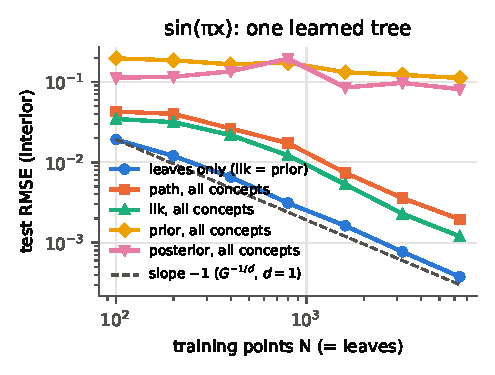
\includegraphics[width=0.48\linewidth]{figs/weighting_sin.pdf}\hfill
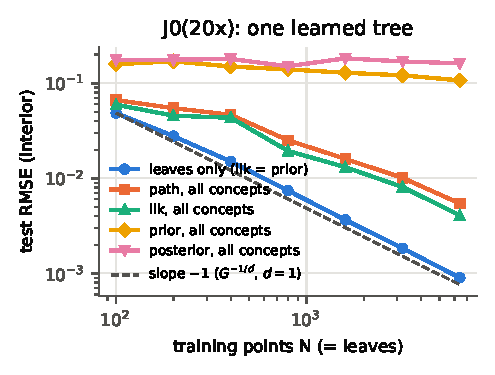
\includegraphics[width=0.48\linewidth]{figs/weighting_j0.pdf}
\caption{One learned tree, variance floor at the data spacing, full expansion.  The
leaves-only mixture falls with slope $-1$; the \textsc{path} and \textsc{lik} mixtures
over all concepts fall more slowly; the \textsc{prior} mixture over all concepts falls only
like $1/\log N$ and the \textsc{posterior} mixture stays high (\cref{rem:hierarchy}).
Numbers in \cref{tab:weighting}.}
\label{fig:weighting}
\end{figure}

\begin{table}[t]
\centering\small
\begin{tabular}{@{}llrrrr@{}}\toprule
target & mixture & $N=100$ & $N=400$ & $N=1600$ & $N=6400$\\\midrule
$\sin(\pi x)$ & leaves only & 0.019 & 0.0066 & 0.0016 & 0.00038\\
$\sin(\pi x)$ & path, all & 0.043 & 0.026 & 0.0074 & 0.002\\
$\sin(\pi x)$ & lik, all & 0.035 & 0.022 & 0.0053 & 0.0012\\
$\sin(\pi x)$ & prior, all & 0.197 & 0.166 & 0.132 & 0.112\\
$\sin(\pi x)$ & posterior, all & 0.113 & 0.135 & 0.085 & 0.081\\
$J_0(20x)$ & leaves only & 0.049 & 0.015 & 0.0037 & 0.0009\\
$J_0(20x)$ & path, all & 0.066 & 0.047 & 0.016 & 0.0054\\
$J_0(20x)$ & lik, all & 0.059 & 0.043 & 0.013 & 0.0041\\
$J_0(20x)$ & prior, all & 0.158 & 0.150 & 0.129 & 0.107\\
$J_0(20x)$ & posterior, all & 0.175 & 0.180 & 0.183 & 0.162\\
\bottomrule\end{tabular}
\caption{Interior test RMSE of one learned tree (mean of three seeds), the data of
\cref{fig:weighting}.}
\label{tab:weighting}
\end{table}

\Cref{fig:weighting,tab:weighting} show the four weightings on learned trees.  These runs
are outside the hypotheses of \cref{thm:single,prop:prior}, which concern a constructed
grid tree, and of \cref{thm:consistency}: the variance floor equals the data spacing
($h\asymp1/N$), the interpolation regime of a noise-free target, not the regime
$Nh^d\to\infty$.  They show the same pattern as the constructions: for $\sin(\pi x)$ the
leaves-only error falls from $0.019$ at $N=100$ to $0.00038$ at $N=6400$, a factor of about
four per quadrupling of $N$, while the \textsc{prior} mixture over all concepts stays
between $0.11$ and $0.20$ and the \textsc{posterior} mixture between $0.08$ and $0.14$ at the tabulated $N$ (and
$0.19$ at $N=800$ in the figure)
(between $0.15$ and $0.19$ for $J_0(20x)$).

\subsection{The KAN battery}

\begin{figure}[t]
\centering
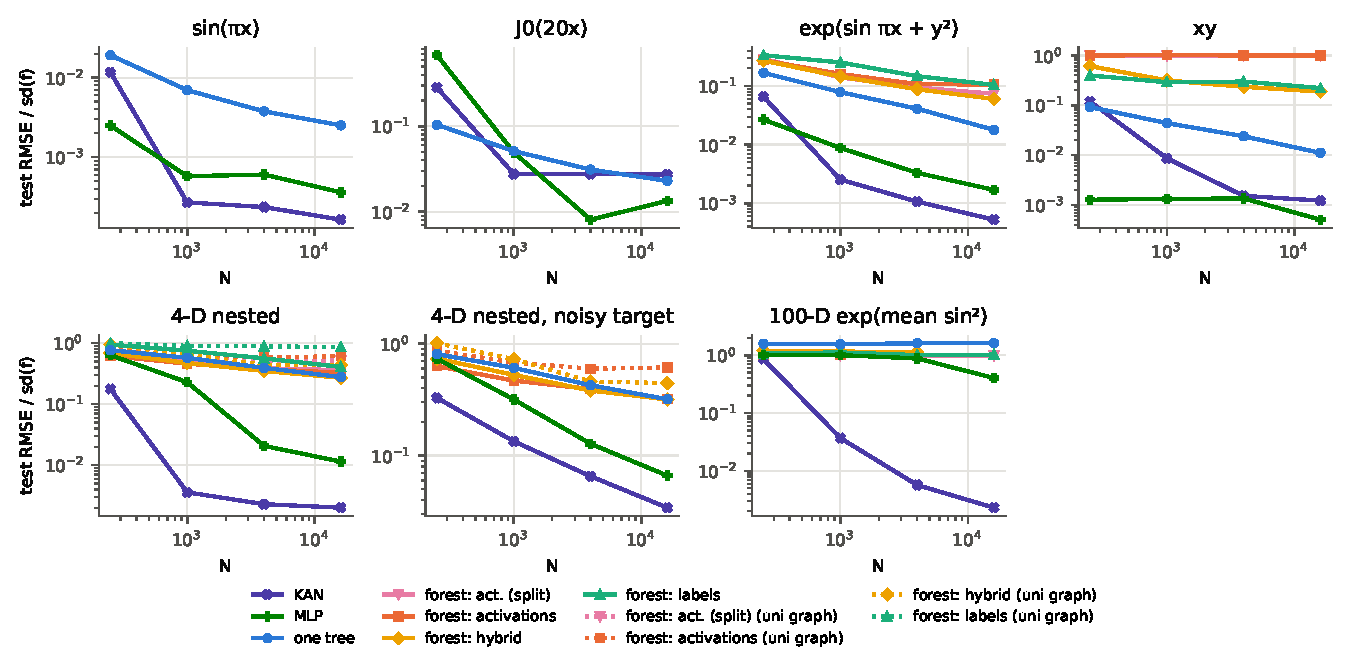
\includegraphics[width=\linewidth]{figs/toys.pdf}
\caption{Test RMSE$/\mathrm{sd}(f)$ against $N$.  Forests are drawn with their best
graph (dotted: the univariate graph of the 4-D target).}
\label{fig:toys}
\end{figure}

\begin{table}[t]
\centering\small
\resizebox{\linewidth}{!}{\begin{tabular}{@{}llrrrrrrr@{}}\toprule
fn & N & one tree & activations & labels & hybrid & act. (split) & MLP & KAN\\\midrule
sin & 250 & 0.019 & -- & -- & -- & -- & 0.003 & 0.012\\
sin & 1000 & 0.007 & -- & -- & -- & -- & 0.001 & 0.000\\
sin & 4000 & 0.004 & -- & -- & -- & -- & 0.001 & 0.000\\
sin & 16000 & 0.002 & -- & -- & -- & -- & 0.000 & 0.000\\
j0 & 250 & 0.104 & -- & -- & -- & -- & 0.681 & 0.283\\
j0 & 1000 & 0.051 & -- & -- & -- & -- & 0.050 & 0.028\\
j0 & 4000 & 0.031 & -- & -- & -- & -- & 0.010 & 0.028\\
j0 & 16000 & 0.026 & -- & -- & -- & -- & 0.014 & 0.027\\
expsin & 250 & 0.167 & 0.274 & 0.334 & 0.271 & 0.289 & 0.027 & 0.065\\
expsin & 1000 & 0.079 & 0.160 & 0.252 & 0.145 & 0.140 & 0.008 & 0.003\\
expsin & 4000 & 0.041 & 0.131 & 0.146 & 0.097 & 0.096 & 0.005 & 0.002\\
expsin & 16000 & 0.018 & 0.186 & 0.114 & -- & -- & -- & --\\
xy & 250 & 0.092 & 1.003 & 0.397 & 0.610 & 0.997 & 0.001 & 0.119\\
xy & 1000 & 0.044 & 1.013 & 0.287 & 0.315 & 1.005 & 0.001 & 0.007\\
xy & 4000 & 0.024 & 1.005 & 0.244 & 0.261 & 1.007 & 0.001 & 0.001\\
xy & 16000 & 0.011 & 1.003 & 0.164 & -- & -- & -- & --\\
nested4 & 250 & 0.765 & 0.618 & 0.946 & 0.685 & 0.695 & 0.663 & 0.056\\
nested4 & 1000 & 0.574 & 0.460 & 0.752 & 0.472 & 0.484 & 0.386 & 0.004\\
nested4 & 4000 & 0.393 & 0.382 & 0.592 & 0.350 & 0.386 & -- & --\\
nested4 & 16000 & 0.277 & 0.347 & -- & -- & -- & -- & --\\
exp100 & 250 & 1.580 & 1.019 & 1.074 & 1.184 & 1.027 & 1.005 & 0.710\\
exp100 & 1000 & 1.001 & 1.001 & 1.151 & 1.171 & 1.023 & 1.006 & 0.036\\
exp100 & 4000 & 0.977 & 0.977 & 1.029 & -- & 0.983 & 0.880 & --\\
exp100 & 16000 & 0.993 & -- & -- & -- & -- & 0.409 & --\\
\bottomrule\end{tabular}}
\caption{The KAN battery: test RMSE$/\mathrm{sd}(f)$, mean of three seeds.  ``activations''
is the funnel forest; for the 4-D target the forests use the pairs graph (superscript
$u$: univariate graph).}
\label{tab:toys}
\end{table}

\Cref{fig:toys,tab:toys} show five things.
(i)~One tree's error falls with $N$ on every target of dimension at most four, the
behaviour \cref{thm:consistency} predicts (the runs use the \textsc{path} mixture with a
budget, outside its hypotheses).  On $\sin(\pi x)$ and $\exp(\sin\pi x+y^2)$ at $N=16000$ it is
7 to 11 times behind the MLP and 16 to 34 times behind the KAN; on $J_0(20x)$ it is ahead of
both at $N=250$ and ahead of the KAN, whose grid limits it, at $N=16000$.
(ii)~On $xy$ the funnel forest stays between $0.99$ and $1.02$ at every $N$---what
\cref{prop:xy} predicts in the limit, under hypotheses (split protocol, count-weighted
full expansion) that these online, budget-limited runs do not meet--- while labels ($0.22$ at $N=16000$) and hybrid
messages ($0.19$) learn; the single tree over both coordinates is better still ($0.011$),
because with $n=2$ it has the same fan-in.
(iii)~On the 4-D target the funnel forest over the pairs $(x_1,x_2),(x_3,x_4)$, which is
sufficient by \cref{prop:suffclass}, beats the single tree at small $N$ ($0.46$ against
$0.57$ at $N=1000$) and loses at $N=16000$ ($0.33$ against $0.28$).  Here $n=k+2$, so the
bounds of \cref{rem:crossover} have equal exponents.  With a noisy target the remark's
bounds favour the forest, which leads at small $N$ ($0.63$ against $0.81$ at $N=250$) but
only ties at $N=16000$ ($0.320$ against $0.319$).  In both cases the measured slopes run the
other way---about $-0.16$ for the forest against $-0.22$ (noisy) and $-0.24$ (noise-free)
for the single tree over $N=250$ to $16000$---so at these sample sizes the comparison is not
governed by the bounds' exponents; the forest's composition error, which the bounds
ignore, is a likely reason that we have not isolated.
(iv)~On the 100-D target no Cobweb design gets below $0.95$ (the single tree is worse
than the constant predictor, at $1.55$ to $1.61$), while the KAN reaches $0.002$ and the
MLP $0.40$.

\begin{table}[t]
\centering\small
\resizebox{\linewidth}{!}{\begin{tabular}{@{}rrrrrrrrrrr@{}}\toprule
$N$ & leaf budget & $\kappa$ & level 0 & level 1 & level 2 & level 3 & level 4 & level 5 & level 6 & output\\
 & & & $|S|{\le}1$ & $|S|{\le}2$ & $|S|{\le}4$ & $|S|{\le}8$ & $|S|{\le}16$ & $|S|{\le}32$ & $|S|{\le}64$ & RMSE/sd\\\midrule
4000 & 100 & 0.25 & 1.38 & 1.42 & 1.40 & 1.27 & 1.12 & 1.08 & 1.02 & 1.00\\
4000 & 100 & 1.0 & 3.16 & 1.46 & 1.41 & 1.38 & 1.19 & 1.08 & 1.06 & 1.01\\
4000 & 1000 & 1.0 & 0.57 & 0.87 & 1.06 & 1.10 & 1.06 & 1.06 & 1.02 & 1.00\\
4000 & 4000 & 1.0 & 0.57 & 0.82 & 0.99 & 1.02 & 1.01 & 1.00 & 1.00 & 1.00\\
\bottomrule\end{tabular}}
\caption{The 100-D funnel forest level by level ($N$ training points, one seed): RMSE
of every tree's activation divided by the standard deviation of its ideal message
$m_S$, averaged over the trees of a level.  A ratio near $1$ means the activation
carries no information about $m_S$.}
\label{tab:diag100}
\end{table}

(v)~\Cref{tab:diag100} locates the 100-D failure.  Each univariate tree must estimate
$\E[Y\mid X_i]$, whose standard deviation is about a tenth of that of $Y$.  At $N=4000$, with a budget
of 100 leaves the estimate is dominated by noise (ratio $1.4$ for $\kappa=0.25$, $3.2$ for
$\kappa=1$); with 1000 or 4000 leaves it carries signal (ratio $0.57$), but the trees one
level up read these noisy activations, and the signal is gone by the third level.  At $N=16000$ with 4000 leaves part of
it survives to the top (ratios $0.56$ to $0.91$, output $0.92$): with this budget the composition improves with $N$, in the direction \cref{thm:ideal}
predicts for the limit, but with 1000 leaves the low levels get worse with $N$ ($0.57\to0.90$
at level~0), so the improvement depends on the budget; these runs are in any case outside
the theorem (online protocol, a budget, and messages with critical points, outside (A2)).  This is the finite-sample face of the
condition behind (A4): the children's errors are not small compared with what their
parents must resolve, and errors compound through the levels.  A KAN does not face this
problem, because its gradient corrects all inner functions against the error of the
output.

\subsection{Cognitive tasks}\label{sec:exp-tasks}

\begin{table}[t]
\centering\small
\begin{tabular}{@{}llrrrrrr@{}}\toprule
& & \multicolumn{2}{c}{tree perceiving $x_2$ alone} & \multicolumn{4}{c}{composing tree (test RMSE)}\\
\cmidrule(lr){3-4}\cmidrule(l){5-8}
$N$ & world & val.\ RMSE & act.\ sd & funnel & labels ($d{=}3$) & hybrid & merged\\\midrule
1000 & $P_a$ & 1.004 & 0.062 & 1.008 & 0.675 & 0.642 & 0.270\\
1000 & $P_b$ & 1.002 & 0.080 & 1.006 & 1.143 & 1.116 & 1.080\\
4000 & $P_a$ & 1.000 & 0.047 & 1.064 & 0.460 & 0.510 & 0.244\\
4000 & $P_b$ & 1.002 & 0.048 & 1.028 & 1.074 & 1.056 & 1.018\\
16000 & $P_a$ & 1.003 & 0.069 & 1.164 & 0.429 & 0.471 & 0.215\\
16000 & $P_b$ & 1.004 & 0.073 & 1.092 & 1.051 & 1.034 & 1.007\\
\bottomrule\end{tabular}
\caption{The two sign worlds of \cref{thm:locality} (five seeds).  Left: a tree that
perceives $x_2$ and predicts $Y$---its validation RMSE equals that of the constant
predictor ($1.00$) and its activation is flat in both worlds.  Right: the composing
tree's test RMSE for four task assignments.}
\label{tab:locality}
\end{table}

\paragraph{Locality.}
\Cref{tab:locality} reproduces \cref{thm:locality} in data: the tree that perceives $x_2$
has the same validation error and the same flat activation in both worlds, so nothing
it can compute tells it whether $x_2$ matters.  The composing tree separates the worlds:
under $P_a$ the merged tree reaches $0.22$ and the label forest $0.43$ at $N=16000$, while
under $P_b$, where $f\equiv0$ and the constant predictor is optimal, every assignment
stays near $1$.  The funnel forest fails under $P_a$, where its error even rises above the constant predictor's ($1.16$ at $N=16000$), because
its online, budget-limited activations are noise that the output tree fits.

\begin{table}[t]
\centering\small
\begin{tabular}{@{}lrlrrr@{}}\toprule
target & $N$ & selected (count of 5) & funnel & selected & best candidate\\\midrule
xy & 500 & merge (5) & 1.020 & 0.071 & 0.071\\
xy & 2000 & merge (5) & 1.000 & 0.032 & 0.032\\
xy & 8000 & merge (5) & 1.003 & 0.019 & 0.019\\
sign & 500 & merge (5) & 0.996 & 0.309 & 0.309\\
sign & 2000 & merge (5) & 1.007 & 0.245 & 0.245\\
sign & 8000 & merge (5) & 1.075 & 0.231 & 0.231\\
expsin & 500 & merge (5) & 0.232 & 0.115 & 0.115\\
expsin & 2000 & merge (5) & 0.145 & 0.055 & 0.055\\
expsin & 8000 & merge (5) & 0.111 & 0.034 & 0.034\\
nested4 & 500 & funnel-pairs (4), funnel (1) & 0.773 & 0.662 & 0.657\\
nested4 & 2000 & funnel-pairs (5) & 0.651 & 0.451 & 0.450\\
nested4 & 8000 & funnel-pairs (3), hybrid-pairs (2) & 0.622 & 0.334 & 0.334\\
\bottomrule\end{tabular}
\caption{Task selection by verification (\cref{thm:selection}; five seeds).  Candidates:
the funnel forest, label forests of depth 2, 3 and 4, a hybrid forest, one merged tree and,
for the 4-D target, funnel and hybrid forests over the pairs.  Columns: how often each
candidate was selected, and the test RMSE$/\mathrm{sd}$ of the funnel forest, of the
selected forest and of the best candidate in hindsight.}
\label{tab:selection}
\end{table}

\paragraph{Selection.}
Selecting by the validation error at the output (\cref{tab:selection}) never selects the
funnel forest on $xy$ or on the sign target.  On the 4-D target it selects a forest over
the pairs in 14 of 15 runs (in one run at $N=500$ it selects the univariate funnel forest),
over the merged 4-D tree.  The selected forest's test error is within one percent of the
best candidate's in every cell.  On two-dimensional targets the merged tree wins, as it
should: it has the same fan-in as the forest and no composition error.  These runs test the selection rule rather than
instantiate \cref{thm:selection}: the theorem assumes that every candidate converges,
whereas here every candidate is trained online with the \textsc{path} mixture and a
budget, and the fixed-depth label and hybrid candidates are not covered by our consistency
results.

\begin{figure}[t]
\centering
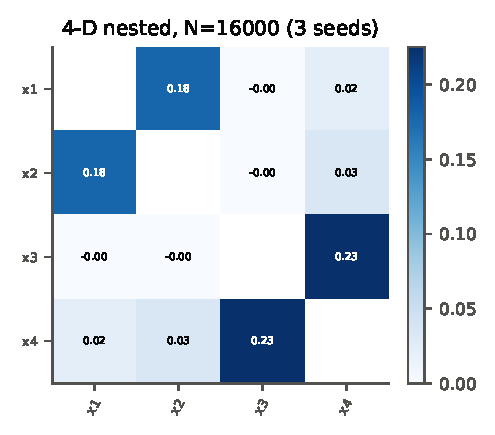
\includegraphics[width=0.92\linewidth]{figs/synergy.pdf}
\caption{Synergy deficits (\cref{def:operators}): validation MSE of the funnel pair forest
minus that of one tree over the pair, divided by $\Var(Y)$.  Left: the 4-D target; the
two blocks stand out and the cross-block deficits are near zero.  Right: California
housing; the largest deficits are longitude--latitude and rooms--bedrooms.}
\label{fig:synergy}
\end{figure}

\paragraph{Synergy.}
\Cref{fig:synergy} estimates the synergy deficit of every pair of coordinates, the
quantity step~2 of \cref{proc:induction} thresholds.  On the 4-D target the within-block
deficits are $0.18$ and $0.23$ of $\Var(Y)$ and the cross-block deficits are within
$0.04$ of zero, so the threshold recovers the blocks $\{x_1,x_2\}$ and $\{x_3,x_4\}$.  On
housing the deficit of longitude with latitude is large in every run ($0.13$ to $0.17$ at
$N=4000$): location is an interaction that activations do not carry.  Rooms with bedrooms
averages $0.13$ in \cref{fig:synergy} but varies between data splits ($-0.01$ to $0.25$), so
the induction runs of \cref{tab:induce}, which estimate their own deficits, mostly leave
it below the threshold.  At $N=16000$ every housing pair shows a positive deficit (between $0.03$ and
$0.22$), so the threshold of step~2 must account for sample size.  The deficit vanishes
whenever both activations are injective functions of their cues, whatever the
interaction (\cref{def:operators}), so a positive deficit marks an interaction that the
activations lose, not every interaction.

\begin{table}[t]
\centering\small
\resizebox{\linewidth}{!}{\begin{tabular}{@{}lrlrrrrr@{}}\toprule
target & $N$ & induced groups ($\tau=0.05$) & one tree & balanced & selected & best & seeds\\\midrule
I.12.11 & 4000 & $\{q\} \{E_f\} \{B,v,\theta\}$ & 0.216 & 0.594 & 0.212 & 0.212 & 3\\
I.13.12 & 4000 & $\{m_1\} \{m_2\} \{r_1\} \{r_2\} \{G\}$ & 0.311 & 0.634 & 0.311 & 0.311 & 3\\
I.29.16 & 4000 & $\{x_1\} \{x_2\} \{\theta_1,\theta_2\}$ & 0.217 & 0.853 & 0.217 & 0.217 & 3\\
I.37.4 & 4000 & $\{I_1\} \{I_2\} \{\delta\}$ & 0.106 & 0.299 & 0.106 & 0.106 & 3\\
I.50.26 & 4000 & $\{x_1\} \{\omega,t\} \{\alpha\}$ & 0.345 & 0.826 & 0.327 & 0.326 & 3\\
I.6.20 & 4000 & $\{\sigma,\theta\}$ & 0.023 & 0.350 & 0.023 & 0.023 & 3\\
I.6.20b & 4000 & $\{\sigma\} \{\theta,\theta_1\}$ & 0.083 & 0.536 & 0.083 & 0.083 & 3\\
I.9.18 & 4000 & $\{m_1\} \{m_2\} \{x_2\} \{x_1\} \{y_2\} \{y_1\} \{z_2\} \{z_1\} \{G\}$ & 0.438 & 0.602 & 0.438 & 0.438 & 3\\
II.6.15a & 4000 & $\{\epsilon,r\} \{p_d\} \{x,y\} \{z\}$ & 0.519 & 0.562 & 0.546 & 0.494 & 3\\
nested4 & 4000 & $\{x_1,x_2\} \{x_3,x_4\}$ & 0.450 & 0.607 & 0.407 & 0.407 & 3\\
nested4 & 16000 & $\{x_1,x_2\} \{x_3,x_4\}$ & 0.300 & 0.626 & 0.294 & 0.294 & 3\\
\bottomrule\end{tabular}}
\caption{Task induction end to end (\cref{proc:induction}; three seeds, $\kappa=0.25$ for
every candidate, so the single-tree errors differ from those of \cref{tab:toys,tab:feynman},
which tune $\kappa$).  Groups formed by step~2 at threshold $\tau=0.05$ (most frequent
over seeds, each run estimating its own deficits) and test RMSE$/\mathrm{sd}$ of the
single tree, of the generic balanced forest over the inputs, of the forest selected on
validation data among the single tree, the balanced forest and the induced forests for
$\tau\in\{0.02,0.05,0.1,0.2\}$ with activation or hybrid messages, and of the best
candidate in hindsight.}
\label{tab:induce}
\end{table}

\paragraph{Task induction.}
\Cref{tab:induce} runs \cref{proc:induction} end to end.  The groups it forms are the
interactions that activations lose: in $q(E_f+Bv\sin\theta)$ it merges $B$, $v$ and
$\theta$ and keeps $E_f$ apart, and it also keeps $q$ apart, although $q$ multiplies every
term, because $q$'s activation is injective; in $I.6.20b$ it merges $\theta$ with
$\theta_1$, whose difference the formula uses; in $I.29.16$ it merges the two angles; on
the 4-D target it recovers the two blocks.  The selected forest equals the best candidate,
or is within one percent of it, in every row but one; it beats the single tree where the
induced structure is real (the 4-D target and housing at both sizes, e.g.\ $0.495$ against
$0.598$ on housing at $N=16000$, where the threshold $\tau=0.05$ merges every input but the
selected forests, at $\tau=0.1$ or $0.2$, merge only longitude with latitude in all three runs;
and narrowly on $I.12.11$ and $I.50.26$); and it falls back
on the single tree on the other formulas.
The exception is $II.6.15a$, where the selected forest ($0.546$) is worse than the single
tree ($0.519$), which was among the candidates.  The generic balanced forest is the worst
design on every formula: a forest needs the right graph, and verification at the
composing tree finds one.

\begin{figure}[t]
\centering
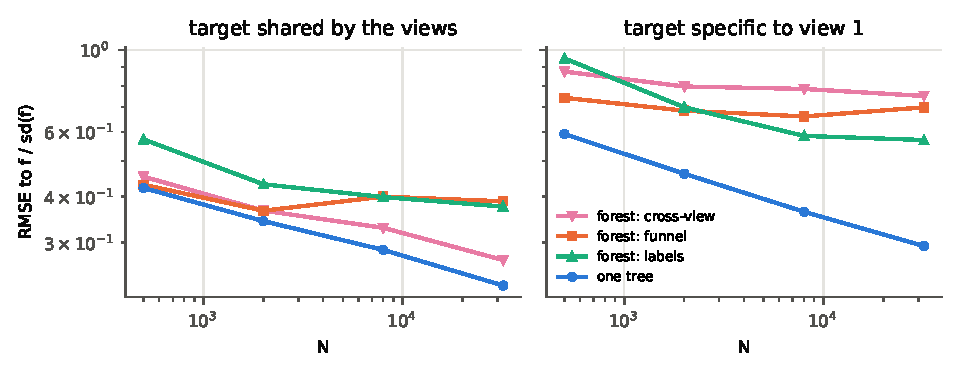
\includegraphics[width=0.85\linewidth]{figs/multiview.pdf}
\caption{The two-view Gaussian model of \cref{prop:multiview} (five seeds): RMSE to the
optimal predictor $f$, divided by $\mathrm{sd}(f)$.  Left: $Y=\sin(2Z)$ depends on the
shared latent.  Right: $Y$ is the first noise coordinate of view 1.}
\label{fig:multiview}
\end{figure}

\paragraph{Cross-view tasks.}
In the two-view model (\cref{fig:multiview}) the cross-view forest, whose inner trees
never see $Y$, keeps improving when the target depends on the shared latent ($0.45$ at
$N=500$, $0.27$ at $N=32000$), as \cref{prop:multiview} predicts, while the funnel forest
stalls near $0.39$: here the funnel messages $\E[\sin2Z\mid X^{(v)}]$ are not invertible
functions of the per-view posterior means, so the funnel assignment is not sufficient.
When the target is specific to one view the cross-view forest stalls near $0.75$: a
positive deficit, as predicted after \cref{prop:multiview} (the remark predicts its sign,
not its size).  The single tree over all four
coordinates is best in both panels at these sample sizes.  (The Gaussian views are
unbounded, so \cref{thm:ideal} itself does not cover these runs.)

\paragraph{Cue calculus.}
\Cref{proc:cues} was run, with the fixed tolerance $\tau=0.02$ and no tuning, on a cue
suite with known kinds---$Y=\sin(\pi x_0)+\operatorname{sign}(x_1x_2)+\varepsilon$ with
$x_0$ associative, $(x_1,x_2)$ a purely contextual pair, $x_3$ irrelevant and $x_4$ a copy
of $x_0$ up to noise of standard deviation $0.01$---and on California housing
(\cref{tab:cues}, five seeds each).  On the suite every cue is classified correctly on every seed:
both copies of $x_0$ are valid, exactly one survives and the other is blocked by it,
the contextual pair has validities within $0.03$ of zero alone and above $0.6$ jointly,
and the forest built from the classification (one tree for the associative cue, one
merged tree for the pair) cuts the test RMSE of the single tree over all cues by a
factor of $2.5$.  On housing the stable part of the classification is the one the
earlier experiments found by hand: income, rooms, longitude and latitude are associative
on every seed, longitude and latitude are merged on four of five, and occupancy is
irrelevant on every seed.  The weak cues (age, bedrooms, population) change kind between
seeds; their validities are within a few multiples of $\tau$ of zero, where the
estimator of step~1 cannot separate the kinds.  The cue forest is selected on four seeds, and on those it
reaches the test RMSE of the hand-designed pairs forest of \cref{tab:housing}
($0.30$--$0.32$ against $0.29$--$0.30$, same splits) without a designer and without a
hyperparameter grid; on the fifth the classification yields one group and the single
tree is kept.  MLP and KAN remain better ($0.26$--$0.28$).
\begin{table}[h]\centering\small
\IfFileExists{tables/cues.tex}{\begin{tabular}{@{}lp{7.6cm}rrr@{}}\toprule
data & cue kinds (superscript: seeds out of all, when not all) & selected & one tree & forest chosen\\\midrule
cue suite & assoc. assoc$^{4}$, copy$^{1}$; context. ctx2, ctx1; blocked copy$^{4}$, assoc$^{1}$; irrel. noise & 0.176 & 0.439 & 5/5\\
housing & assoc. income, lat, lon, rooms, pop$^{1}$; context. bedrooms$^{3}$, age$^{2}$, pop$^{1}$; blocked pop$^{3}$, bedrooms$^{1}$, age$^{1}$; irrel. occup, age$^{2}$, bedrooms$^{1}$ & 0.566 & 0.649 & 4/5\\
\bottomrule\end{tabular}}{}
\caption{\Cref{proc:cues}: modal cue kinds over five seeds, and test RMSE$/\mathrm{sd}(Y)$ of the
selected model and of one tree over all cues ($\kappa=0.25$, $N=3000$ for the suite and
$N=4000$ for housing).}\label{tab:cues}
\end{table}

\subsection{Continual learning, interpretability and labels}

\begin{figure}[t]
\centering
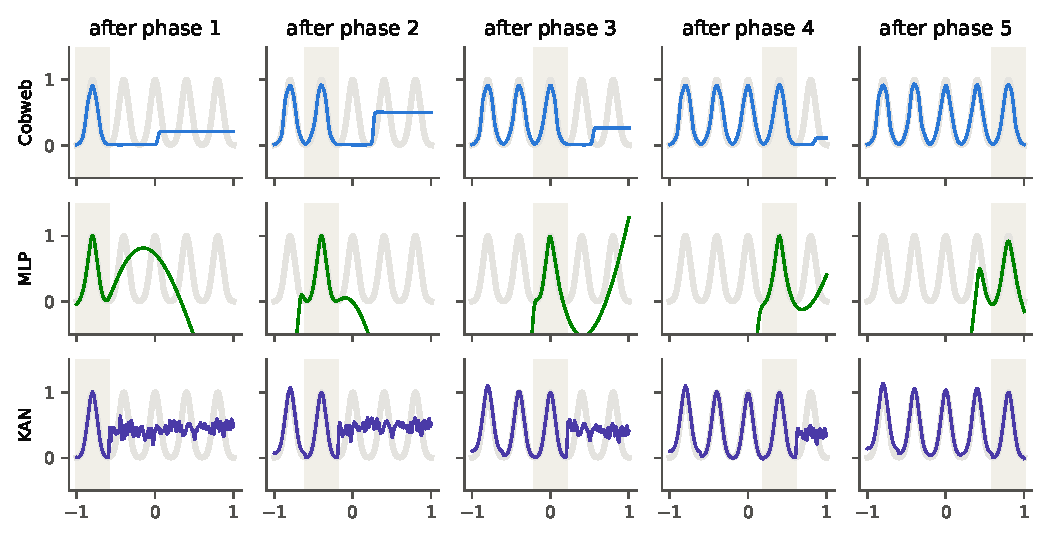
\includegraphics[width=0.9\linewidth]{figs/continual.pdf}
\caption{The continual-learning task of \citet[Fig.~3.4]{liu2024kan}: five peaks, one
region per phase (shaded).  Grey: target.}
\label{fig:continual}
\end{figure}

\begin{table}[t]
\centering\small
\begin{tabular}{@{}lrrrrr@{}}\toprule
method & \multicolumn{5}{c}{RMSE on all data seen so far, after phase 1..5}\\\midrule
cobweb & 0.037 & 0.048 & 0.045 & 0.045 & 0.045\\
mlp & 0.014 & 0.965 & 10.756 & 7.506 & 8.241\\
kan & 0.009 & 0.107 & 0.161 & 0.160 & 0.168\\
\bottomrule\end{tabular}
\caption{Continual learning: RMSE on all data seen so far after each phase (three seeds).}
\label{tab:continual}
\end{table}

\paragraph{No forgetting.}
\Cref{lem:leaves} says that nothing a tree has learned is deleted.  On the KAN paper's
continual task (\cref{fig:continual,tab:continual}) the tree's error on everything seen
so far stays between $0.037$ and $0.048$ through all five phases; the MLP forgets
(its error reaches $10.8$), and the KAN with a fine grid forgets partly ($0.17$).

\begin{figure}[t]
\centering
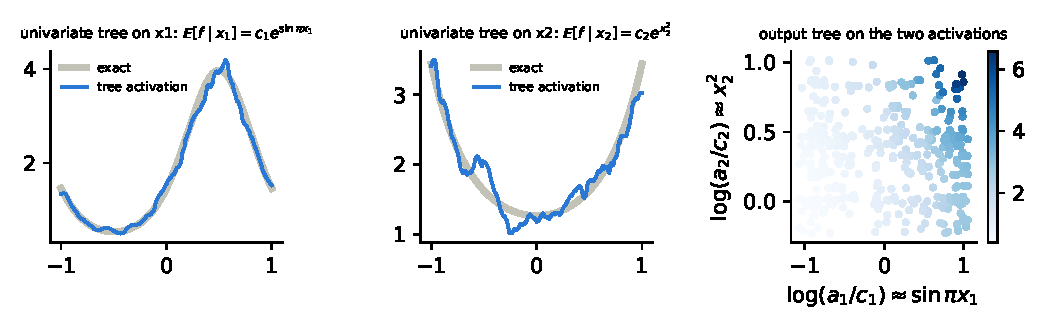
\includegraphics[width=\linewidth]{figs/interpret.pdf}
\caption{What the univariate trees of a funnel forest learn on $\exp(\sin\pi x_1+x_2^2)$
($N=4000$).  Left and centre: each tree's activation against the exact conditional
expectation $\E[f\mid x_i]$.  Right: the output tree's prediction as a function of the
two activations.}
\label{fig:interpret}
\end{figure}

\paragraph{Interpretability.}
A KAN's edges can be plotted, and so can a Cobweb forest's trees.  On
$\exp(\sin\pi x_1+x_2^2)$ the univariate trees learn $c_1e^{\sin\pi x_1}$ and $c_2e^{x_2^2}$
(\cref{fig:interpret}), the inner functions of the target up to the monotone maps
$H_S$ of \cref{prop:suffclass}, without gradients.

\begin{figure}[t]
\centering
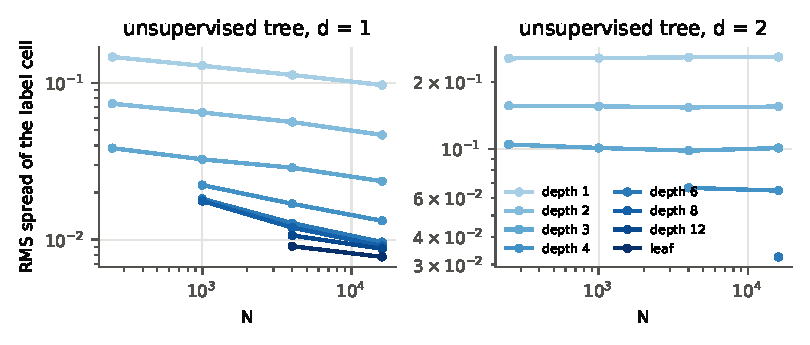
\includegraphics[width=0.8\linewidth]{figs/label_cells.pdf}
\caption{Spread of the cell of a label at fixed depth, for unsupervised trees over
uniform data.}
\label{fig:cells}
\end{figure}

\paragraph{Label cells.}
\Cref{thm:labelcons} needs the cells of the labels to shrink.  In one dimension the cells
of a fixed depth shrink slowly as the tree grows; in two dimensions they do not
(\cref{fig:cells}).  Labels become fine enough only if their depth grows with $N$; the
depths our experiments try are fixed ($2$ to $6$), so the label forests of this section
are outside \cref{thm:labelcons}.  We also tried the cognitively attractive choice of the
\emph{basic level}---the concept of largest expected pointwise mutual information on the
branch, which Cobweb computes: for continuous attributes it lies near the leaves (mean
depth $10$ to $11$), because a concept's information grows as its variance shrinks
towards the variance floor, and its labels did worse than any fixed depth on $xy$.

\subsection{Real data}

\begin{table}[t]
\centering\small
\resizebox{\linewidth}{!}{\begin{tabular}{@{}lrrrrrrr@{}}\toprule
equation & $n$ & single & act & label & hybrid & mlp & kan\\\midrule
I.12.11 & 5 & 0.140 & 0.592 & 0.578 & 0.479 & 0.004 & \textbf{0.002}\\
I.13.12 & 5 & 0.281 & 0.626 & 0.916 & 0.492 & 0.006 & \textbf{0.005}\\
I.29.16 & 4 & 0.182 & 0.854 & 0.880 & 0.422 & \textbf{0.011} & 0.095\\
I.37.4 & 3 & 0.092 & 0.257 & 0.360 & 0.206 & \textbf{0.003} & 0.003\\
I.50.26 & 4 & 0.308 & 0.801 & 0.871 & 0.793 & \textbf{0.016} & 0.125\\
I.6.20 & 2 & 0.021 & 0.339 & 0.097 & 0.094 & 0.001 & \textbf{0.001}\\
I.6.20a & 1 & 0.002 & -- & -- & -- & 0.000 & \textbf{0.000}\\
I.6.20b & 3 & 0.078 & 0.511 & 0.605 & 0.541 & \textbf{0.003} & 0.020\\
I.9.18 & 9 & 0.322 & 0.476 & 0.891 & 0.573 & \textbf{0.003} & 0.015\\
II.6.15a & 6 & 0.486 & 0.556 & 0.878 & 0.421 & \textbf{0.013} & 0.024\\
\bottomrule\end{tabular}}
\caption{Feynman equations, $N=4000$: test RMSE$/\mathrm{sd}(f)$, mean of three seeds;
forests use a balanced graph over the inputs in their listed order.}
\label{tab:feynman}
\end{table}

\begin{table}[t]
\centering\small
\resizebox{\linewidth}{!}{\begin{tabular}{@{}lrrrrrrrrr@{}}\toprule
N & single & act:pairs & act:uni & label:uni & label:pairs & hybrid:uni & hybrid:pairs & mlp & kan\\\midrule
1000 & 0.362$\pm$0.009 & 0.336$\pm$0.011 & 0.366$\pm$0.002 & 0.535$\pm$0.009 & 0.464$\pm$0.027 & 0.408$\pm$0.016 & 0.357$\pm$0.011 & 0.308$\pm$0.009 & 0.286$\pm$0.008\\
4000 & 0.325$\pm$0.006 & 0.299$\pm$0.005 & 0.344$\pm$0.005 & 0.496$\pm$0.035 & 0.461$\pm$0.005 & 0.339$\pm$0.012 & 0.314$\pm$0.008 & 0.271$\pm$0.005 & 0.262$\pm$0.004\\
16000 & 0.303$\pm$0.002 & 0.276$\pm$0.003 & 0.346$\pm$0.006 & 0.496$\pm$0.014 & 0.432$\pm$0.008 & 0.314$\pm$0.005 & 0.279$\pm$0.009 & 0.250$\pm$0.001 & 0.249$\pm$0.002\\
\bottomrule\end{tabular}}
\caption{California housing: test RMSE of the log median value (three seeds).}
\label{tab:housing}
\end{table}

\begin{table}[t]
\centering\small
\begin{tabular}{@{}lrrrrrr@{}}\toprule
N & single & label & act & hybrid & mlp & kan\\\midrule
1000 & 83.2$\pm$1.1 & 70.7$\pm$1.7 & 85.8$\pm$0.3 & 84.7$\pm$0.1 & 88.2$\pm$1.1 & 88.6$\pm$0.6\\
5000 & 91.4$\pm$0.4 & -- & -- & -- & 94.0$\pm$0.2 & 92.2$\pm$0.7\\
20000 & -- & -- & -- & -- & 96.8$\pm$0.3 & 94.5$\pm$0.7\\
\bottomrule\end{tabular}
\caption{MNIST, accuracy (\%, three seeds).  Forests have one tree per $7\times7$
patch.  ``label'': the patch trees categorize (the Convolutional-Cobweb protocol);
``cross'': they predict the centre pixels of the neighbouring patches; ``act'': they
predict the class and pass its distribution; ``hybrid'': ``act'' plus labels.}
\label{tab:mnist}
\end{table}

\begin{table}[t]
\centering\small
\begin{tabular}{@{}lrr@{}}\toprule
N & ngram & mlp\\\midrule
20000 & 17.8 / 5.07 & 20.9 / 5.10\\
100000 & 19.1 / 4.84 & 21.7 / 4.66\\
300000 & 19.9 / 4.68 & 23.6 / 4.41\\
\bottomrule\end{tabular}
\caption{Next word on OpenWebText from the previous four words (2000-word vocabulary):
top-1 accuracy (\%) / cross-entropy (nats).  An accuracy of 20.9 is the frequency of the
unknown-word token.}
\label{tab:owt}
\end{table}

\paragraph{Feynman equations.}
With a balanced graph over the inputs in their listed order---a graph that ignores the
structure of each formula---the forests lose to the single tree on every equation except
$II.6.15a$, where the hybrid forest is better ($0.421$ against $0.486$; \cref{tab:feynman}).
The MLP and the KAN are better than every Cobweb design on every equation, by factors from
about two (the single tree against the KAN on $I.29.16$) to more than a hundred.
\Cref{tab:induce} shows that \cref{proc:induction} finds structure in the formulas and
matches or beats the single tree on every equation but $II.6.15a$; it does not close the
gap to the gradient-trained models.

\paragraph{Housing.}
The funnel forest over the natural pairs (longitude--latitude, age--rooms,
bedrooms--occupancy, households--income) beats the single tree at every $N$
($0.276$ against $0.303$ at $N=16000$; \cref{tab:housing}), and the univariate graph
does not; the pairs graph keeps together longitude and latitude, the strongest
interaction of \cref{fig:synergy}.  MLP and KAN are better still.

\paragraph{MNIST.}
Patch trees that predict the class and pass their predicted class distributions beat the
single tree over all pixels at $N=1000$ and $5000$ and match it at $20000$ ($94.4\pm0.5$
against $94.2\pm0.3$), and the hybrid forest reaches $94.9\%$ at
$N=20000$, level with the KAN ($94.5\%$) and below the MLP ($96.8\%$; \cref{tab:mnist}).
Categorizing patch trees (the Convolutional-Cobweb protocol) are weaker than
outcome-predicting ones at every $N$ ($70.7\%$ to $86.2\%$): categorization alone passes
less information about the class than outcome prediction does.  Patch trees that predict
the centre pixels of their neighbouring patches---perceptual prediction, which never sees
the class---are the weakest design ($37\%$ to $52\%$ on average).  A plausible reading, which we have
not tested, is that the class is not what neighbouring centre pixels share---the analogue
of the multi-view redundancy that \cref{prop:multiview} assumes in its Gaussian
setting---so the activations discard most of what identifies the digit.

\paragraph{Text.}
On next-word prediction (\cref{tab:owt}) the trees' most probable word is the unknown-word
token, so their accuracy equals its frequency, and their cross-entropy is worse than that
of an interpolated $n$-gram; at $N=20000$ the funnel label forest improves the single tree's
cross-entropy slightly ($5.77$ against $5.88$; the unsupervised one does not, $5.87$), and
neither improves its accuracy.  A Cobweb language
model needs the architecture of a dedicated study; we report these numbers as the limit
of the generic forest.

%=====================================================================
\section{Discussion}\label{sec:discussion}
%=====================================================================

\paragraph{A cognitive reading.}
The three task families of \cref{def:task} are three things a learner can do with what it
perceives: \emph{categorize} it, \emph{predict an outcome} of it, or \emph{predict
another part of it}.  The first is concept formation in Cobweb's original sense; the
second is cue--outcome learning \citep{rescorla1972}; the third is the perceptual
prediction of predictive-processing accounts \citep{clark2013}.  Each has a mathematical
counterpart here.  Categorization is sufficient whenever its cells shrink, stay few compared with the
sample, and its smoothing vanishes fast enough, and it pays for every cell it distinguishes (\cref{thm:labelcons,rem:tradeoff}):
its categories must become finer with experience, just as the activations' consistency
needs the variance floor---the acuity---to shrink, $h_N\to0$; both are perceptual learning
in the sense of \citet{goldstone1998}.  Outcome prediction
compresses the cue to what matters for the outcome, which is sufficient when the
outcome depends on the parts monotone-additively (\cref{prop:suffclass}) and can fail on
interactions (\cref{prop:xy}).  Perceptual prediction never needs the target and, in a
Gaussian latent model, is sufficient when the target depends only on what the views
share (\cref{prop:multiview}).

\paragraph{Credit assignment.}
\Cref{thm:locality} is a precise form of the credit-assignment problem
\citep{minsky1961}: a module cannot learn its role from the statistics it sees when the
information it carries is synergistic.  Back-propagation solves the problem by sending
the composed error to every module.  A Cobweb forest has no error signal, and the theory
says where the decision must be taken instead: at the tree that composes the parts, by
verifying candidate tasks against an observed outcome (\cref{thm:selection}).  The
locality and selection experiments show both halves.

\paragraph{Rules of thumb for composing trees.}
The results suggest a small set of rules for building a forest whose trees use one
another's representations.
\begin{enumerate}[leftmargin=*,noitemsep]
\item \emph{Give every tree an observable outcome or none.}  A tree can learn only what
  it will observe (\cref{def:task,rem:kaobs}); inner functions of a target are not tasks.
\item \emph{Pass activations where the parts combine monotonically, labels or a merged
  cue where they interact.}  Funnel activations are sufficient for monotone-additive
  targets (\cref{prop:suffclass}) and fail on $x_1x_2$ and on parity
  (\cref{prop:xy,cor:parity}); a positive synergy deficit (\cref{def:operators}) is the
  measurable sign that two cues must be merged or passed as labels.
\item \emph{Decide a tree's task where its message is used.}  A tree's own data cannot
  tell whether its cue matters (\cref{thm:locality}); compare candidate tasks by the
  held-out or prequential error of the composing tree (\cref{thm:selection}), and always
  keep the merged tree among the candidates (\cref{proc:induction}).
\item \emph{Use perceptual prediction only when the target lives in what the views
  share.}  Cross-view outcomes need no target and are sufficient under that condition
  (\cref{prop:multiview}); on MNIST, where neighbouring pixels do not carry the class, they
  were the weakest design (\cref{tab:mnist}).
\item \emph{Keep categories few and let them sharpen with experience.}  Label cells must
  shrink and stay few compared with the data (\cref{thm:labelcons}); a fixed label depth
  does neither.
\item \emph{Keep forests shallow.}  Two inputs per tree suffice in principle
  (\cref{thm:cka}), but every level of composition adds error that the next level reads
  as noise (\cref{tab:diag100}).
\item \emph{Predict with counts and train predict-then-learn.}  Count-blind mixtures fail
  on repeated instances (\cref{rem:counts}); messages computed in-sample leak the target
  (\cref{def:forestlearn}).
\end{enumerate}

\paragraph{Limitations.}
\Cref{thm:ideal} covers the split protocol with full expansion, exact matching and the
count-weighted leaves-only mixture; the experiments use the online protocol, a leaf
budget, the implementation's tolerance and the \textsc{path} mixture, which the theory
does not cover (\cref{rem:counts,rem:structure}).  Step~2 of the proof of
\cref{thm:ideal} relies on standard uniform laws for kernel sums rather than a full
derivation, the conditions of \cref{thm:labelcons} on the label cells are not derived
from category utility, and the hybrid case is a conjecture (\cref{conj:hybrid}).
\Cref{proc:induction} is greedy and its thresholds are not calibrated.  Finally, the
rates are those of nonparametric smoothing: on smooth targets gradient-trained models
are far more accurate, and in high dimension a funnel forest's errors compound through
its levels (\cref{tab:diag100}).

\appendix
%=====================================================================
\section{Verification}\label{app:verify}
%=====================================================================

\paragraph{Executable verifier.}
\texttt{verification/checks.py} instantiates the objects each statement talks about with
the real C++ tree---learned by \texttt{ifit}, or built exactly for the constructions in
the proofs (depth-one grid trees, the label-forest construction, interwoven trees)---and
tests the statement's conclusion; \texttt{verification/run.py} writes the table below.
The first check compares \cref{def:predict} and \cref{def:concept}, implemented from the
definitions, with the code's scores and mixtures.

\IfFileExists{tables/verification.tex}{\begin{center}\small\begin{tabular}{@{}llp{9.2cm}@{}}\toprule
result & statement & check\\\midrule
pass & \cref{def:predict} & Def.~multi-node prediction and Def.~concept equal the implementation\\
pass & \cref{lem:leaves} & Leaf preservation (no leaf deleted; additivity; leaves hold identical copies)\\
pass & \cref{lem:bias} & Concept-bias certificate holds for every weighting and budget\\
pass & \cref{thm:single}, \cref{prop:prior} & Grid tree: error and root weight vanish (lik, path, leaves); prior plateaus\\
pass & \cref{thm:label} & Label-forest construction meets its error bound; labels are nearest grid points\\
pass & \cref{prop:interweave} & Interwoven tree = convex combination of the subtrees (lik, path)\\
pass & \cref{lem:dag}, \cref{thm:cka} & Composed constructed trees approximate $\Phi(\varphi_1+\varphi_2)$\\
pass & \cref{thm:consistency} & Learned tree, leaves-only lik = Nadaraya--Watson (path is not)\\
\textbf{fail} & \cref{check_xy} & check_xy\\
pass & \cref{thm:locality} & Sign construction: local laws equal; composition separates the worlds\\
pass & \cref{prop:multiview} & Posterior given all views = function of per-view posterior means\\
pass & \cref{rem:structure} & Branch-and-bound stop returns a sub-optimal concept\\
\bottomrule\end{tabular}\end{center}}{}

\paragraph{Formal proofs.}
The discrete cores of the statements below are proved in Lean~4 with Mathlib
\citep{moura2021lean4,mathlib2020} (\texttt{lean/}, built by \texttt{lake build}).  The
check \texttt{check\_lean} rebuilds the project, prints the axioms of every listed theorem and
fails if any depends on \texttt{sorryAx} or if a source file contains \texttt{sorry},
\texttt{admit} or a new \texttt{axiom}; every theorem uses only Lean's standard axioms
(\texttt{propext}, \texttt{Classical.choice}, \texttt{Quot.sound}).
\begin{center}\small
\begin{tabular}{@{}lp{5.6cm}p{6.2cm}@{}}\toprule
statement & Lean theorem & scope\\\midrule
\cref{prop:cues}(a) & \texttt{validity\_nonneg}, \texttt{condExp\_const\_of\_validity\_zero} & any finite distribution and cue\\
\cref{prop:cues}(b) & \texttt{condExp\_blocked}, \texttt{conditional\_validity\_blocked} & any finite distribution, any $f$\\
\cref{thm:locality}(i)--(ii) & \texttt{sign\_worlds\_local\_law}, \texttt{local\_rule\_same}, \texttt{sign\_worlds\_differ} & the sign skeleton on $\{\pm1\}^3$\\
\cref{cor:parity} & \texttt{parity\_fibre\_balanced} & parity of all $n$ bits ($J=[n]$, signs as bits), every $S$ missing a bit\\
\cref{prop:interweave} & \texttt{merged\_prediction}, \texttt{merged\_weights} & the mixture identity, $m$ subtrees\\
\cref{prop:fanin} & \texttt{Chain.fanin\_one} & every fan-in-one forest\\
\cref{thm:cka} (count) & \texttt{ka\_tree\_count} & $4n^2+4n$ trees, $n\ge1$\\
\bottomrule
\end{tabular}
\end{center}
Analytic statements (rates, consistency) are not formalised; for them the executable
checks and the review below carry the verification.

\paragraph{Adversarial review.}
Each statement is also checked by an independent reviewer---a fresh language-model agent
for every round---instructed to break it, to settle questions by computation, and to
read nothing but this document, its tables and the two C++ files it formalises
(\texttt{verification/REVIEW\_PROMPT.md}).  The reviewer was calibrated before it was
trusted: on a copy of an earlier draft with eight planted errors (three of them real
mistakes of that draft) it found all eight with correct diagnoses, and every other flag it
raised was a genuine error, which we fixed.  The same prompt was then run on successive
drafts:

\begin{center}\small
\begin{tabular}{@{}lp{11.5cm}@{}}\toprule
round & outcome\\\midrule
calibration & 8/8 planted errors found; extra findings (label consistency with atoms, exact matching, crossover exponents) fixed\\
2 & no statement false under its hypotheses; experiments text contradicting tables, overstated remarks and summaries; fixed\\
3 & no statement false under its hypotheses; prior/posterior weightings on hierarchies (verified by check C19), branch-and-bound repair, minor gaps; fixed\\
4 & no statement invalid; four minor gaps (an unsatisfiable form of a hypothesis of \cref{thm:labelcons}, an unused density hypothesis, a cited uniform law, an ambiguous phrase) and five text items; fixed\\
\bottomrule
\end{tabular}
\end{center}

\noindent The reports, the drafts they reviewed and the reviewers' own scripts are in
\texttt{verification/reviews/}; how each finding was resolved is in
\texttt{verification/REVIEW.md}.

\bibliographystyle{plainnat}
\bibliography{refs}
\end{document}
